\documentclass{article}
\usepackage{graphicx} % Required for inserting images

\usepackage{subcaption}
\usepackage{subcaption}
\usepackage{float}
\usepackage{dialogue}
\usepackage{tikz}
\usepackage{natbib}
\usepackage{setspace}
\usepackage{tabularx}

\usepackage{amsmath}
\usepackage{amsthm}
\usepackage{amssymb}
\usepackage{tcolorbox}


%%%%%%%%%%%%%%%%%%%%
% For appendix math formulas
\theoremstyle{plain}
    \ifx\thechapter\undefined
      \newtheorem{lem}{\protect\lemmaname}
    \else
      \newtheorem{lem}{\protect\lemmaname}[chapter]
    \fi
\theoremstyle{plain}
    \ifx\thechapter\undefined
  \newtheorem{cor}{\protect\corollaryname}
\else
      \newtheorem{cor}{\protect\corollaryname}[chapter]
    \fi
\providecommand{\corollaryname}{Corollary}
\providecommand{\lemmaname}{Lemma}
%%%%%%%%%%%%%%%%%%%%


\DeclareMathOperator{\CostBlock}{CostBlock}
\newtheorem{theorem}{Theorem}
\newtheorem{proposition}[theorem]{Proposition}
\newtheorem{definition}[theorem]{Definition}
\DeclareMathOperator{\minCost}{minCost}

\begin{document}
%\title{The Economics of Generative and Agentic AI}
% John's footnote: \footnote{I used AI extensively to write this paper, particularly Claude 3.5 Sonnet and o1 pro from OpenAI. Thanks for complementing my labor, AI agents!}
\title{AI, Tasks and Judgement}
\author{\normalsize John J. Horton  \\ \normalsize MIT \& NBER  \and \normalsize Peyman Shahidi \\  \normalsize MIT}
\date{\today{}}



\newcommand{\machine}[1]{\langle #1 \rangle}
\newcommand{\human}[1]{( #1 )}
\newcommand{\cost}[1]{C\{ #1 \}}
\newcommand{\costdo}[1]{C_H\{ #1 \}}
\newcommand{\costmanage}[1]{C_M\{ #1 \}}
\newcommand{\tasktime}[1]{t_{#1}}
\newcommand{\taskhc}[1]{c_{#1}}
\newcommand{\labor}[1]{l_{#1}}

\newcommand{\topic}[1]{\paragraph{#1}}
%\newcommand{\topic}[1]{#1}

\maketitle

\begin{abstract}
\noindent This paper presents a simple task-based model of Agentic AI and human labor.
The model focuses on the decision to use an AI for a task based on the cost of human prompting and evaluation versus the cost of human performance. 
Unlike other tasks models, it considers the interdependence of tasks in a sequence. 
Tasks can be efficiently ``chained'' together in the sense that each task produces something that feeds into the next without human intervention.
A task might be added to an automated chain even if the human has an absolute advantage in that task in isolation, reversing the usual comparative advantage calculation.
Furthermore, where investments should be make in AI that can minimize costs depends on the timeline of the investment and can have surprising dyanmics, such as abruptly stopping work to focus on tasks that are still far away from automation.
\end{abstract}

\onehalfspacing
  
\section{Introduction}
We present a simple task-based model of agentic AI and human labor that focuses on the interdependence of tasks in the productive process rather than the content of the tasks.
We start with a model of production that is a sequence of tasks that must be done in order.
Those tasks require human capital to perform, but differ in how long they take to complete.
They also differ in how easily they can be ``handed-off'' from one worker to the next.
This model is used to develop a model of the division of labor in production.
%To have a theory of what collection of tasks AI will do, we need what humans will do.

There are, of course, numerous economic models of the division of labor \citep{becker1992division, deming2017growing}---why do we need another, especially one that is not as analytically tractable as more stylized models?
The short answer is that because AI cannot easily be characterized as a fall in the cost of ``X'', we need to get into the micro-details of the production process: more stylized models cannot easily be paired with engineering estimates focusing on the content of the tasks. 
Second, if we hope to do some kind of comparative statics, we need to have a model of production and jobs with and without an AI that reflects the actual change in capabilities.
Right now, we have AIs now that can do \emph{certain} tasks in minutes (and eventually miliseconds) that a skilled human would have needed a week to perform. 
These can be done at essentially zero marginal cost. 
% (but perhaps hundreds or thousands of dollars in average cost)
% These are not marginal changes. 
% And yet there are other, seemingly similar tasks an AI cannot do.
%If we want to guide technological development, we need to understand the returns to investing in specific AI capabilities.

After developing the model of production, we consider how the development of AI that can do certain tasks changes the division of labor.
In the model, the decision to use an AI is based on comparing two costs: the cost of having a human direct and evaluate the AI's output (which depends on the capabilities of the AI at that particular task) versus the cost of having the human do the task directly.
This might seem like another way of stating that tasks get assigned to whichever factor has the comparative advantage in that task, but this is not the case: the position of tasks within the productive process profoundly change the optimal allocation of tasks between humans and machines.

%This in turn changes the returns to investing in various AI capabilities both statically and dynamically.
When a single task is performed by an AI, there is a human asking for the task to be done and evaluating the output.
But with two or more tasks it is also possible to re-configure production so that an AI completing one task passes the output into the next task, without human intervention.
This chaining is potentially a source of large productivity gains, \emph{but} it requires powerful AIs that can do each task with a high probability of success. 
The model's basic setup shares conceptual similarities to the the o-ring model of production \citep{kremer1993}; the role humans play in the model as offering judgment is consistent with the emphasis in \cite{agrawal2019exploring}.

A key implication of the model is that the possibility of chaining automated tasks together can reverse comparative advantage assignments for individual tasks. 
It can be efficient to use an AI for a task even if humans have a comparative advantage in that task in isolation, because of chaining.
A surprising implication of chaining is that improvements in AI capabilities for a seemingly unrelated task can cause a focal task to go directly from being done by human to being done by machines.

Because of chaining, it matters what tasks are ``next'' to each other in a productive process.
In different occupations, different tasks might appear adjacent to each other. 
Writing might appear next to hundreds of different tasks, from ``send your economics paper to a journal'' at the end of a semester without teaching, to ``drop your maintence report slip into a box'' at the end of a shift driving a bus.
As such, ``automation dispersion'' is a possibility where tasks are automated in some production settings but not others because of occupation-specific task adjacency.

Assigning tasks to factors of production is not a competely trivial computational problem.
For an occupation with $n$ tasks, we show that there are $F(2n + 1)$ possible production arrangements, where $F(k)$ is the $k$th Fibonacci number.
However, we also show how the allocation problem can be solved numerically in $O(n^2)$ time using dynamic programming.
Although we do not do it in this paper, this algorithmic approach could be combined with micro-details of task content and composition (as in \cite{frey2017future, felten2021occupational, eloundou2023gpts}) to create rich estimates of how technological change in various tasks would impact workers. 

Beyond just the allocation of tasks to factors of production, the model provides a way to calculate the return to investing in AI capabilities in specific tasks.
For tasks far from economical automation (i.e, done by humans), marginal investments in AI capabilities offer no immediate return.
Once capabilities exceed the threshold where AI replaces humans even in isolation, improvements in AI capabilities offer a return, but at a diminishing rate.
But once the chaining threshold is passed, the returns to investing in AI for that focal task discontinuously increase.
These non-linearities in the returns to investment in AI creates interesting optimal investment path dynamics, which we explore in the $n = 2$ case.

In the $n = 2$ task case, with a high discount rate, it can be optimal to invest heavily in a single AI capability, leaving the other task to always be done by humans.
With a low discount rate, the optimal path can change dramatically. 
As with other growth models, there is a ``get on the turnpike'' effect: the optimal path is to invest heavily in AI for the lagging task until it reaches parity with the more advanced task, with both of them chained, after which we have balanced investment across AI tasks.
Depending on the starting point, before getting on the turnpike, it is sometimes optimal to continue to invest in the leading task for some amount of time, in order to enjoy lower costs while getting the lagging task up to parity.
Although we present this investment path as attempting to minimize total costs, other objectives are possible, such adding a constraint such a labor income not falling too quickly.

The chaining feature of the model connects to---and potentially reconciles---competing views about automation in production. 
Despite the emphasis on task-level substitution between AI and labor in most of the AI and labor literature \citep{autor2003skill, acemoglu2018automation}, \cite{bresnahan2002information} argues that that meaningful substitution happens primarily at the system level. 
One could interpret the model as showing how task-level decisions aggregate into system-level automation through chaining.
In the model, there is no ship-of-theseus requirement that tasks are automated one by one but rather than entire chains can be automated all at once---consistent with the \cite{bresnahan2002information} perspective.

Although the model is developed as a kind of algorithmic cost function, it ultimately produces cost functions with standard properties, which we embed within a more general model of the economy.  
The model predicts that improvements in AI will inherently reduce labor use per unit of the good and, consequently, its price.  
Whether this increases or decreases the demand for labor, even for that task, depends on the elasticity of demand for that good in the product market.  
Further complicating things, if AI has wide-ranging effects, changing the cost of many goods at once, then a partial equilibrium analysis that ignores income effects or cross-price elasticities would be insufficient, even setting aside the change in task composition from new goods and services.
This limitation suggests the need for complementary empirical work tracking the evolution of tasks and occupations as AI capabilities advance.

In the model, with highly capable AIs, the human role shrinks to asking and judging. 
This perhaps sounds like an uninspiring role---and perhaps less enjoyable role \citep{toner2024artificial}---but it is not necessarily a low-paid one. 
Consider the famed music producer Rick Rubin, who is not poor, discussing his market value in an interview with Anderson Cooper:
\begin{dialogue}
    \speak{Rick Rubin} I've no technical ability. And I know nothing about music.
    \speak{Anderson Cooper} Well, you must know something.
    \speak{Rick Rubin} I know what I like and what I don't like. I'm decisive about what I like and what I don't like.
    \speak{Anderson Cooper} So what are you being paid for?
    \speak{Rick Rubin} The confidence that I have in my taste, and my ability to express what I feel, has proven helpful for artists.
\end{dialogue}
We might be paid for being hepful to AIs.
And this help might be valuable, even if we have no ability to do the tasks ourselves.
In other words, automation can enable new forms of labor-labor substitution by separating task execution from task evaluation, allowing workers to leverage judgment skills even in domains where they lack execution abilities, potentially upending the allocation of workers to occupations in hard-to-forsee ways (see \cite{autor2013putting} on this human capital-task-wage relationship).
Given the Rubin example, one might imagine that AI might enable a super-star phenomenon, but as with so many of these questions, it likely depends on the product market elasticity of demand for the output.

% Most empirical work on AI and labor market has implitly adopted this focus, examining the actual content of the tasks and technical capabilities of machines, as determined by engineering or expert estimate \citep{frey2017future, felten2021occupational, eloundou2023gpts}; 
% This work has also kept with the framing of task-based models as a bundle of tasks, without considering the structural relationship between tasks \citep{autor2003skill, acemoglu2018automation}.

%Why are there still so many jobs \citep{autor2015}?


\section{A General Equilibrium Model with Task-Based Production}
\label{sec:taskbased_GE}

\subsection{Task-Based Production}
Consider an economy with $K$ final goods.
A single (representative) firm produces and trades all goods under perfect competition in separate markets.
For each good $k \in \{1,\ldots,K\}$, production requires completing an ordered set of tasks, denoted by:
\[
\mathcal{T}_k = \{1,2,\ldots,\tau_k\}.
\]
We refer to $\mathcal{T}_k$ as the production process for good $k$.
For ease of exposition, we focus on a representative sector and omit the subscript $k$ from our notation until subsection~\ref{sec:household_GE}.
This simplification means that when we refer to variables or production processes, they implicitly pertain to a typical final good.

The firm can partition the production process $\mathcal{T}$ into a number of ``jobs,'' where each job is a contiguous block of tasks performed by a single worker.
With $|\mathcal{T}| = \tau$ tasks, there are $2^{(\tau - 1)}$ unique ways of designing jobs.
For example, if $\tau = 3$, the production process of the final good consists of three tasks, $\{1,2,3\}$, with $2^{(3-1)}=4$ unique job designs.
Let $[.]$ denote the tasks assigned to a worker in a job.
The four possible designs in this example are: $\{[1][2][3], \, [1,2][3], \, [1][2,3], \, [1,2,3]\}$.
The second design, for instance, implies that one worker is assigned to do tasks 1 and 2 in a single job, $[1,2]$, whereas task 3 is assigned to a different worker in another job, $[3]$.

Next, we formalize the definition of jobs for an arbitrary number of tasks and an arbitrary number of jobs.
Suppose the firm breaks down the production process $\mathcal{T}$ into $J$ jobs.
Let $i_j$ denote the first task in job $j \in \{1,\ldots,J\}$ in the production process of the final good.
We can write:
\[
1 = i_1 < i_2 < \cdots < i_{J+1} = \tau+1.
\]
This means that the first task is the first task of the first job, $i_1=1$, while the (imaginary) task $\tau+1$ is considered the first task of the (imaginary) job $j = J+1$.
With this notation, the $j$th job can be characterized as a collection of consecutive tasks in the production process $\mathcal{T}$:
\[
\mathcal{J}_j = \{i_j, \, i_j+1, \, \cdots, \, i_{j+1} - 1\}.
\]
Going back to the earlier example with $\tau=3$, the four potential job designs can formally be expressed as:
\begin{align*}
\{[1][2][3]\} \Longleftrightarrow \ J = 3:  & \quad \mathcal{J}_1 = \{1\}, \quad  \mathcal{J}_2 = \{2\}, \quad \mathcal{J}_3 = \{3\}, \\
\{[1,2][3]\} \Longleftrightarrow \ J = 2: & \quad \mathcal{J}_1 = \{1, 2\},  \quad \mathcal{J}_2 = \{3\}, \\
\{[1][2,3]\} \Longleftrightarrow \ J = 2: & \quad \mathcal{J}_1 = \{1\}, \quad \mathcal{J}_2 = \{2, 3\}, \\
\{[1,2,3]\} \Longleftrightarrow \ J = 1: & \quad \mathcal{J}_1 = \{1,2,3\}.
\end{align*}

Assume that the worker employed in job $j$ produces an intermediate good $x_j$ and sells it to the firm in a perfectly competitive market.
The firm buys all intermediate goods $\{x_1, \cdots, x_J\}$ from workers and produces the final good at no additional cost using a Leontief production function:
\[
x(x_1, \cdots, x_J) = min\{x_1, \cdots, x_J\}.
\]
This implies that, in equilibrium, the amount of final good $x$ produced is the same as the amount of each intermediate good $x_j$ used in production of the final good.
This is merely a technical assumption reflecting the fact that to produce one unit of the final good, each set of tasks in $\mathcal{T}$, across all jobs $j \in \{1,\ldots,J\}$, must be performed exactly once.
We also assume that tasks in $\mathcal{T}\!$ are performed in fixed proportions.
For instance, if task $m \in \mathcal{T}$ takes 30 minutes and task $n \in \mathcal{T}$ (with $m \neq n$) takes 45 minutes, then producing one unit of good $k$ requires a total of 75 minutes spent on $m$ \underline{and} $n$ as both tasks must be performed exactly once; it is not possible to perform task $m$ multiple times while performing task $n$ only once.
We postpone formalizing this assumption until when we characterize the equilibrium.

In order to produce the intermediate good $x_j$ a worker must complete the tasks associated with that job, namely $\mathcal{J}_j$.
Each task $i \in \mathcal{J}_j$ necessitates acquiring human capital $\taskhc{ij} > 0$ and takes time $\tasktime{ij} > 0$ to complete.
The worker incurs the human capital cost for task $i$ only once at the beginning of his tenure at job $j$, but spends time $\tasktime{ij}$ completing task $i$ for producing each unit of intermediate good $x_j$. 
In other words, having acquired the necessary human capital, the production of each unit of intermediate good uses labor as the only input.
The total human capital acquired ex ante by the worker employed in job $j$ is:
\[
\sum_{i \in \mathcal{J}_j} \taskhc{ij},
\]
while the total time he spends on tasks in $\mathcal{J}_j$ to produce one unit of output is:
\[
\sum_{i \in \mathcal{J}_j} \tasktime{ij}.
\]

Both the product and human capital markets are perfectly competitive, and workers are \emph{ex ante} identical, as in \cite{becker1992division}.
Workers value leisure at $v_L$ and supply one unit of labor inelastically.
To remain indifferent between jobs, workers must receive compensation that accounts not only for the value of their time but also for any additional training costs.
Thus, the wage rate in job $j$ must satisfy\footnote{Notice that while wages may differ across jobs, they are structured to ensure that workers remain indifferent to acquiring different types of human capital for different jobs.}:
\[
w_j = v_L + \sum_{i \in \mathcal{J}_j} \taskhc{ij}.
\]
The firm must pay workers for their time, regardless of the task; hence, the wage bill paid to worker per unit of good $x_j$ is:
\[
\text{WageBill}_j = \Biggl(v_L + \sum_{i \in \mathcal{J}_j} \taskhc{ij} \Biggr) \Biggl(\sum_{i \in \mathcal{J}_j} \tasktime{ij} \Biggr).
\]

Without additional frictions, the firm could minimize the cost of production by assigning a single worker to each task.
What prevents this is a ``hand-off cost''---a cost tied to job transitions that, while not requiring additional human capital, does take time.
This can be interpreted as the cost of context-switching (or hand-off) between workers in the production process.
Specifically, whenever a job boundary is introduced---that is, when transitioning from the last task of job $j$ to the first task of job $j+1$---the worker in job $j$ incurs a hand-off time cost $\tasktime{hj} \geq 0$.

The firm seeks to minimize the total cost of producing the final good by optimally designing jobs while taking hand-off costs into account.
Assuming there are $J$ jobs in the optimal design, the overall production cost per unit of final good is:
\[
\text{TotalCost} = \sum_{j=1}^J \Biggl[\Biggl(v_L + \sum_{i \in \mathcal{J}_j} \taskhc{ij} \Biggr) \Biggl(\tasktime{hj} + \sum_{i \in \mathcal{J}_j} \tasktime{ij} \Biggr)\Biggr].
\]

The firm's problem has a nice geometric interpretation, as shown in Figure~\ref{fig:job_design}.
The productive process is represented as a sequence of stacked rectangles of height $\taskhc{ij}$ and width $\tasktime{ij}$.
A job corresponds to the bounding box around a sequence of tasks---including the hand-off---with its wage bill given by the area of that box.
Note that each rectangle can also be thought of as a series of smaller tasks (smaller rectangles filling in the larger rectangle).
At the limit, this would become a smooth curve of tasks.
Panel (a) of Figure~\ref{fig:job_design} shows a potential job design for a sequence of 7 tasks, while panel (b) shows all 64 possible job designs
\begin{figure}[htbp]
  \begin{center}
  \caption{Example allocations of workers to tasks when $\tau = 7$} \label{fig:job_design}
  \begin{subfigure}[b]{0.48\textwidth}
    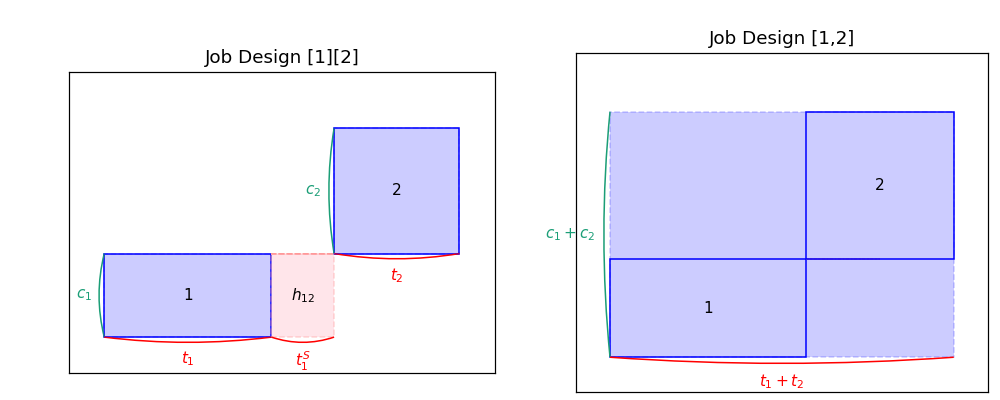
\includegraphics[width=\textwidth]{plots/job_design.png}
    \caption{Allocation of $\tau=7$ task production to $J = 3$ workers}
  \end{subfigure}
  \hfill
  \begin{subfigure}[b]{0.48\textwidth}
    \includegraphics[width=\textwidth]{plots/combined_grid.png}
    \caption{All possible allocations of $\tau=7$ task production}
  \end{subfigure}
  \end{center}
  \footnotesize{Notes: This figure shows potential job designs for a sequence of 7 tasks.
  The total cost of each job is given by the area of its bounding box, which includes the area of the switching cost rectangles (shaded in pink).
  }
\end{figure}



\subsection{AI Facilitates Hand-off}
Here we discuss what determines the hand-off cost introduced in previous part.
Again for simplicity, let us suppress the job-specific notation $j$ until the very last part of this subsection.
All the parameters discussed here implicitly pertain to a typical job.

Suppose the worker can do the hand-off in one of two ways: manually or using an AI.
If he does so manually, he must spend time $\tasktime{w} \geq 0$ to hand off the output of the job.
However, the worker also has access to an AI technology that can perform the same hand-off for a time cost $\tasktime{m} \geq 0$ with success probability $q$.
The expected cost of using the AI to handle the hand-off is:
\[
\tasktime{m} \Bigg( \sum_{\ell=1}^{\infty} \ell q (1 - q)^{\ell - 1} \Bigg) = \frac{\tasktime{m}}{q}.
\]
If the worker deploys the AI instead of handing off the job manually, he incurs an additional time cost equal to $\alpha \geq 0$ times the AI’s hand-off cost.
This represents the cost of AI \emph{management} that the worker must bear, with $\alpha$ reflecting the worker's management efficiency.
A high value of $\alpha$ implies that managing the AI is very costly, whereas a lower value indicates that the AI deployment cost is relatively small (with $\alpha = 0$ meaning the hand-off is effectively free when using AI).
The decision of whether to deploy the AI depends on whether the manual hand-off cost exceeds the AI management cost.
In particular, the worker manages the hand-off using AI if and only if the AI management cost is less than the manual hand-off cost, i.e.,
\[
\tasktime{w} \geq \frac{\alpha \, \tasktime{m}}{q},
\]
or, equivalently, when the AI is “efficient enough”:
\[
q \geq \frac{\alpha \, \tasktime{m}}{\tasktime{w}}.
\]
The optimal hand-off time at the end of each job is thus:
\[
\tasktime{h} = \min\Bigl\{\frac{\alpha \, \tasktime{m}}{q},\, \tasktime{w}\Bigr\}.
\]
By convention, the hand-off cost for the last task is zero since no hand-off occurs after the final job.
The parameter $\tasktime{hj}$ appearing in the firm's job design problem above is the minimum of manual and AI hand-off cost for job $j$.


\subsection{Consumption} 
\label{sec:household_GE}
A representative household supplies one unit of labor inelastically and has a CES utility function over the $K$ final goods.
Here we bring back the sector notation $k$ to distinguish between final goods the household consumes. The household's utility is:
\[
U(x_{1}, \ldots, x_{K}) = \Bigl(\sum_{k=1}^{K} \delta_k \,x_k^{\tfrac{\sigma - 1}{\sigma}}\Bigr)^{\tfrac{\sigma}{\sigma-1}},
\quad
0 < \delta_k < 1,
\quad
\sum_{k=1}^{K} \delta_k = 1,
\quad
\sigma > 0,
\]  
where $x_k$ denotes final good $k$.
Goods are substitutes if $ \sigma > 1$, complements if $0 < \sigma < 1$, and $\sigma = 1$ corresponds to the Cobb-Douglas case.  
The household faces budget constraint:  
\[
\sum_{k=1}^K p^k \,x_k = I,
\]  
where $p^k$ is price of final good $k$ and $I$ is the total income earned from supplying labor to different jobs across all sectors.  
The income, $I$, is the total sum of earnings from producing intermediate goods, which the household takes as given when choosing how much of each final good to consume.


\subsection{Equilibrium}
Let $k \in \{1, \cdots, K\}$ index sectors (or final goods) and $j \in \{1,\cdots, J_k \}$ index jobs within sectors.
Denote total labor employed in sector $k$ with $L_k$.
Equilibrium prices $\big\{ \big\{ w_j^k, p_j^k \big\}_{j=1}^{J_k} \big\}_{k=1}^K$ are: 
\begin{align*}
\labor{j}^k =  \tasktime{hj}^k + \sum_{i \in \mathcal{J}_j^k} \tasktime{ij}^{k},
& \qquad
w_j^k =  v_L + \sum_{i \in \mathcal{J}_j^k} \taskhc{ij}^{k}, 
& \qquad
p_j^k = w_j^k \labor{j}^k, \\
\labor{}^k = \sum_{j=1}^{J_k} \labor{j}^k,
& \qquad
w^k = \frac{\sum_{j=1}^{J_k} w_j^k \labor{j}^k}{\sum_{j=1}^{J_k} \labor{j}^k},
& \qquad
p^k = w^k \labor{}^k,
\end{align*}
and equilibrium allocations $\big\{ x_k^*, L_k^* \big\}_{k=1}^K$ are:
\begin{align*}
x_k^* = \frac{R_k}{\sum_{\ell=1}^K \labor{}^\ell\,R_\ell},
& \qquad
L_k^* = \labor{}^k\,x_k^* = \sum_{j=1}^{J_k} \labor{j}^k\,x_k^*,
\end{align*}
where
\[
R_k = \Bigl(\frac{p^1}{p^k} \cdot \frac{\delta_k}{\delta_1}\Bigr)^{\sigma}.
\]
The model implies that the job design in production process $\mathcal{T}_k$ (and thus human capital and time costs of tasks) determines $p^k$ and $\labor{}^k$, thereby fully determining the consumption bundle $\{x_k^*\}$ and the labor allocations $\{L_k^*\}$ in equilibrium.
Appendix~\ref{app:GE} gives the full derivation details and further discusses comparative statics with respect to task automation.




\subsection{Adding AI} \label{sec:model}
Now consider a worker completing some sequence of tasks as part of their designed job.
For a single task, we will drop the index. 
As before, they can do the task themselves, at a time cost of $t$.
Let us call that cost $c_h$.

If they choose to use an AI, the human asks the AI to perform the task with a ``prompt''---a request to the model. 
Prompting costs them $c_{p}$.
The AI tries to perform the task, generating output.
That output is then evaluated by the worker at a cost to them of $c_{e}$.
The human can evaluate perfectly.

After we evaluation, we learn if the AI succeeded or failed.
The AI produces the output with a probability $q$, failing with a probability $1-q$.
If the AI fails, the human can provide a new prompt and evaluate a new attempt, incurring costs $c_p$ and $c_e$ again.
Let $c_m = c_p + c_e$ denote the total ``management'' costs associated with using the AI.
Figure~\ref{fig:flow} shows this process graphically.

\begin{figure}[h]
  \centering
  \caption{Using AI to complete a task} \label{fig:flow}
  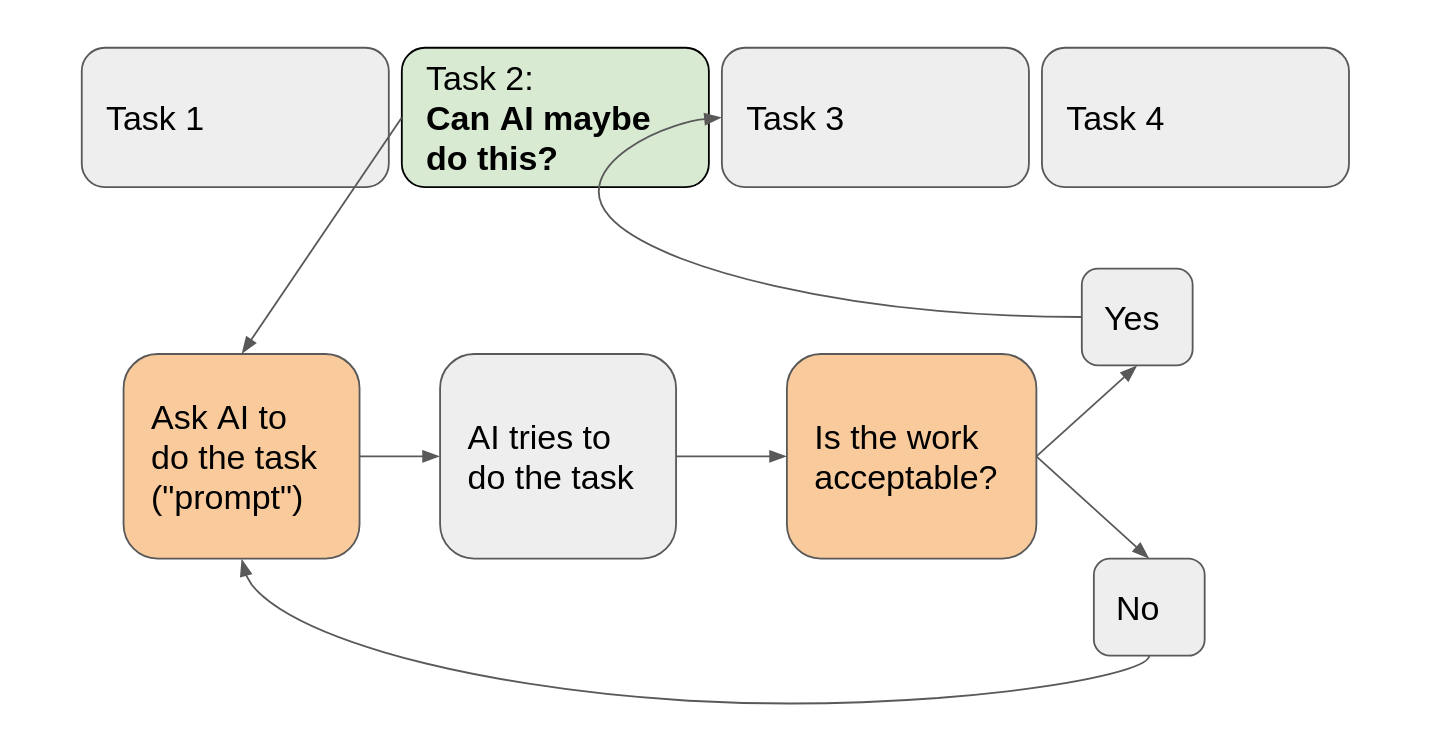
\includegraphics[width = \textwidth]{images/flow.png}
  \footnotesize{Notes: This figure illustrates the iterative process of using AI to complete a task. The human provides a prompt, the AI generates output, and the human evaluates whether the output meets their needs. If not, the process repeats with a refined prompt.}
\end{figure}

Success or failure attempts are assumed to be independent, leading to the following simple Proposition~\ref{proposition:single}.

\begin{proposition}[Single Task Automation Criterion] \label{proposition:single}
A job with a single task should be automated if and only if AI quality exceeds the threshold $\underline{q} := c_m / c_h$.
\end{proposition}
\begin{proof}
The expected cost of using the AI is:
\begin{align*}
    \cost{\machine{1}} &= c_m \sum_{k=1}^{\infty} k q(1-q)^{k-1} \\
    &= c_m/q
\end{align*}
where the second line follows from the standard result for the expectation of a geometric distribution.
Therefore, automation is optimal when $c_m/q < c_h$.
\end{proof}

This criterion has intuitive comparative statics: automation becomes more attractive when human performance costs are high, management costs are low, and the AI's success probability is high.
One implications is that improvements in tools for prompting and evaluation that lower human costs can reduce management costs and thus make automation more attractive, even if the AI's success probability is unchanged.

Independent success probabilities and constant management costs might seem to be strong assumptions, but they are fairly weak and can largely be handled by a re-definition of a parameter e.g., if outcomes are positively correelated, we can treat as-if the success probability is lower. 
See Section~\ref{sec:correlated_successes} for a discussion of correlated success probabilities and see Section~\ref{sec:constant_management_costs} for a discussion of constant management costs.

\subsection{Two task production with the possibility of chaining}
Now we move from a single task to two tasks.  
Although we will eventually consider longer sequences of tasks, most of the important points of the model can be illustrated with just two tasks.

For notation, when a human performs the task, we denote this as $\human{\cdot}$.
When an AI attempts the task under human supervision, we denote this as $\machine{\cdot}$.
For a multiple task example, if the first task was done by AI and the other two by humans, we would write $\machine{1}\human{2}\human{3}$.

The AI success probabilities are $q_1$ and $q_2$ and $c_h$ and $c_m$ are the same for both tasks, for simplicity.
With two tasks, there are four possible direct production arrangements:
\begin{align*}
    \cost{\human{1}\human{2}} &= 2c_h & \text{(fully human)} \\
    \cost{\machine{1}\human{2}} &= \frac{c_m}{q_1} + c_h & \text{(partial automation)} \\
    \cost{\human{1}\machine{2}} &= c_h + \frac{c_m}{q_2} & \text{(partial automation)} \\
    \cost{\machine{1}\machine{2}} &= \frac{c_m}{q_1} + \frac{c_m}{q_2} & \text{(independent automation)}. \\
\end{align*}

There is a fifth arrangement where the completed first task is used as input for the second task without human intervention.
When tasks are chained, denoted by $\machine{1|2}$, they are executed by the AI with a single prompt and final evaluation.
Both tasks must succeed for the chain to be successful in a single step.
The cost of this arrangement is:
\begin{align*}
\cost{\machine{1|2}} &= \frac{c_m}{q_1q_2} & \text{(chained automation)}.
\end{align*}
This captures the notion of agentic AI that can complete a sequence of tasks autonomously, without human intervention between the two tasks.
If $c_h$ and $c_m$ are common across tasks, the full cost function for this productive arrangement when costs are minimizedis thus: 
\begin{align}
  \min \left\{2c_h, 2 \frac{c_m}{q_1}, \frac{c_m}{q_1} + c_h, c_h + \frac{c_m}{q_2}, \frac{c_m}{q_1q_2} \right\}.
\end{align}
Note that as each term is linear in $c_m$ and $c_h$, the cost function itself is convex in labor costs. 

Figure~\ref{fig:two_tasks} shows the cost-minimizing production arrangement for different levels of $q_1$ and $q_2$, with fixed $c_h = 3$ and $c_m = 1$.
It partitions the $q_1$ and $q_2$ space into five regions, corresponding to the five production arrangements.
The ratio of $\underline{q} := c_m / c_h$ is the threshold for automating a task alone.
Interior to this $\underline{q}$-box, we strictly have human production for both tasks, or $\human{1}\human{2}$.
Investing in $q_1$ and $q_2$ offers no immediate return in the $\human{1}\human{2}$ region.
However, once either task is automated, we gain from increasing AI quality further, but at a diminishing rate, so long as the other task is still done by humans.
These regions are the $\machine{1}\human{2}$ and $\human{1}\machine{2}$ regions.

\begin{figure}
  \caption{Cost-minimizing production arrangements with two tasks with levels of AI capabilities} \label{fig:two_tasks}
  \begin{center}
  \includegraphics[width = 0.8 \textwidth]{plots/two_tasks.pdf} \\
  \end{center}
\begin{footnotesize}
  \emph{Note:} This contour plot shows the cost-minimizing production arrangement for different levels of $q_1$ and $q_2$.
  The regions are $\human{1}\human{2}$ (both done by humans), $\machine{1}\machine{2}$ (both done by AI), $\machine{1}\human{2}$ (Task 1 done by AI, Task 2 done by human), $\human{1}\machine{2}$ (Task 1 done by human, Task 2 done by AI), and $\machine{1|2}$ (both tasks done by AI, and chained).
\end{footnotesize}
\end{figure}

The most interesting region is $\machine{1|2}$.
Note that its boundaries with the half-automated regions (e.g., $\machine{1}\human{2}$ and $\human{1}\machine{2}$) are sloped, meaning that improvements in one task's AI quality can bring it into the $\machine{1|2}$ region, without an intervening partial automation step.

This curved boundary is the reason chaining can be optimal even when humans have a comparative advantage in one of the tasks in isolation, as formalized in Proposition~\ref{proposition:interdependence}.
It can shown simply with a numerical example.

\begin{proposition}[Task Interdependence] \label{proposition:interdependence}
A task might be optimally automated as part of a chain even when humans have a comparative advantage in that task in isolation.
Specifically, $\cost{\human{1}\machine{2}} < \cost{\machine{1}\machine{2}}$ does not imply $\cost{\human{1}\machine{2}} < \cost{\machine{1|2}}$.
\end{proposition}
\begin{proof}
Consider $q_1 = 3/5$, $q_2 = 4/5$, $c_m = 1$, and $c_h = 3/2$.
For task 1 in isolation, human performance is cheaper: $c_h = 3/2 < 5/3 = c_m/q_1$.
However:
\begin{align*}
    \cost{\human{1}\machine{2}} &= c_h + \frac{c_m}{q_2} = \frac{3}{2} + \frac{5}{4} = \frac{11}{4} \\
    \cost{\machine{1|2}} &= \frac{c_m}{q_1q_2} = \frac{25}{12} < \frac{11}{4}
\end{align*}
Thus, chaining is optimal despite human comparative advantage in task 1.
\end{proof}

\subsection{General equilibrium in the two-task case}
If there is only one consumption good produced in the $n=2$ case, in equilibium, the firm has to earn zero profit. 
As such, price has to equal marginal cost so $p = w L_{min}$. 
Normalizing the price to $1$, we have $w = \frac{1}{L_{min}}$.
We immediately see that cost-reductions increase the real wage and consumption, despite being whole labor-saving. 

\subsection{Comparative statics of investment in AI capabilities}
The returns to investment in AI for a particular task are affected by AI capabilities in other tasks.
Before a task is automated, there is no return to investment in an AI that does that task.
Once a task is automated, there are returns to investment in a task, but these are unaffected by the other task's AI capabilities.
Once we move into the $\machine{1|2}$ region, the returns to investment in one task are affected by the other task's AI capabilities.
The cost reduction gets steeper immediately when switching into the $\machine{1|2}$ region but then flattens out, as the second derivative of the cost function with respect to $q_i$ is positive.
These properties are formalized in Proposition~\ref{prop:comparative_statics}.

\begin{proposition}[Comparative Statics] \label{prop:comparative_statics}
  The effect of improving AI capabilities has the following properties:
  \begin{enumerate}
  \item In human-only production, improvements in AI have no effect on costs:
  \[\frac{\partial \cost{\human{1}\human{2}}}{\partial q_i} = 0 \text{ for } i \in \{1,2\}\]
  \item In independent AI production, improvements reduce costs independently:
  \[\frac{\partial \cost{\machine{1}\machine{2}}}{\partial q_i} = -\frac{c_m}{q_i^2}, \quad \frac{\partial^2 \cost{\machine{1}\machine{2}}}{\partial q_1 \partial q_2} = 0\]
  \item In mixed production, only improvements in the specific task matter:
  \[\frac{\partial \cost{\machine{1}\human{2}}}{\partial q_1} = -\frac{c_m}{q_1^2}, \quad \frac{\partial \cost{\machine{1}\human{2}}}{\partial q_2} = 0\]
  \item In chained production, improvements are complementary:
  \[\frac{\partial \cost{\machine{1|2}}}{\partial q_i} = -\frac{c_m}{q_i^2q_j}, \quad \frac{\partial^2 \cost{\machine{1|2}}}{\partial q_1 \partial q_2} = \frac{c_m}{q_1^2q_2^2} > 0\]
  where $j \neq i$.
  \end{enumerate}

  In chained production, improvements in AI capabilities eventually flatten out, as the second derivative of the cost function with respect to $q_i$ is positive.
  \begin{equation}
      \frac{\partial^2}{\partial q_1 \partial q_2} \cost{\machine{1|2}} = \frac{c_m}{q_1^2q_2^2} > 0
  \end{equation}

\end{proposition}
 
We will later consider the more general $n$ task case, but note that immediate adjacency is not required for a task where humans have a comparative advantage to be pulled into a chain.
Consider a scenario with $n$ tasks, each with the same success probability $q$ and the same $c_m$ and $c_h$.
To start, all are done by humans, implying that $n c_h < c_m / q^n$.
Now suppose we can increase the $q$ of the first task by $\delta q$. 
If it is possible that  
\begin{align}
  \delta q > \frac{c_m}{n q^{n-1}} - q,
\end{align} 
then all tasks will be done by machine, in one chain.

\subsection{Optimal investment paths in the two-task case}
A natural question is how firms or a social planner should allocate R\&D effort to improve AI capabilities.
In the two task case, rather than taking $q_1$ and $q_2$ as given, we can consider the optimal investment paths, or allocation of R\&D effort.
Suppose we can improve $q_1$ and $q_2$ at a rate $r$ per unit of time.
It we have $T$ periods, then 
\[
\begin{aligned}
\text{Choose } &q_1(\cdot), \; q_2(\cdot) \quad \text{for } t \in [0, T]\\
\text{to minimize } &
   \int_{0}^{T}
   e^{-\rho t} C\bigl(q_1(t), q_2(t)\bigr) \, dt \\[1em]
\text{subject to:} & \\[-1em]
&(1)\quad q_1(0) = q_{1,0}, \quad q_2(0) = q_{2,0}, \\[6pt]
&(2)\quad q_1'(t) + q_2'(t) \le r, \quad \text{for almost all } t \in [0, T], \\[6pt]
&(3)\quad q_1(t) \geq 0, \quad q_2(t) \geq 0, \quad \forall t \in [0, T], \\[6pt]
\end{aligned}
\label{eq:dp_problem}
\]
where $q_{1,0}$ and $q_{2,0}$ are the initial AI capabilities in the two tasks.
The properties of the optimal paths for this dynamic programming problem are analyzed in detail in Appendix~\ref{app:dp_proof}. 
There, we outline the structure of the solution, provide comparative statics, and derive the necessary conditions for optimality.

Figure~\ref{fig:optimal_paths} shows numerical optimal investment paths to minimize total costs, using the same parameters as in Figure~\ref{fig:two_tasks}.
I also set the discount rate $\rho = 0$ and the total amount of R\&D resources per period  to $r = 1$.
I discretized the $q_1$ and $q_2$ space into a grid (so investments had to be made each period on one task or the other) and then used dynamic programing to find the optimal path.
Paths for a few select initial conditions are shown.

\begin{figure}
  \begin{center}
  \caption{Optimal investment paths to minimize costs} \label{fig:optimal_paths}
  \label{fig:optimal_paths} 
  \includegraphics[width = 0.8 \textwidth]{plots/optimal_paths.pdf}
  \end{center}
  \begin{footnotesize}
  \emph{Note:} This plot shows the optimal investment paths to minimize costs, using the same parameters as in Figure~\ref{fig:two_tasks}, with a number of different initial conditions.
\end{footnotesize}
\end{figure}

We can see that the optimal path has a ``turnpike'' component where we move towards the 45 degree line and then make equal investments in $q_1$ and $q_2$.
However, it does not typicaly go there directly but, if already in a semi-automated region, it will increase capabilities in that task for some time, taking advantage of the relatively steep slope. 
In the $\machine{1|2}$ region, the optimal path is to directy move towards the 45 degree line.

\subsection{Investment horizon effects}
The investment horizon can have important effects on the optimal path.
Figure~\ref{fig:horizon_effects} illustrates this by choosing about the same starting positions, but varying the number of steps $T$ in the dynamic program.
As in Figure~\ref{fig:optimal_paths}, a dynamic program is used to find the optimal path that minimizes costs.

We can see that time horizons can create fundamental differences in the optimal path.
With a relatively short horizon, the optimal path is simply to keep investing in the already-automated task.
The reason is that with this horizon, we never get to the $\machine{1|2}$ region.
With a longer horizon, we just keep going farther in $q_1$, neglecting $q_2$.
With a long-enough horizon, we actually stop work on $q_1$ and begin working on $q_2$.
This is despite the fact that $q_2$ offers no benefit at this region.
However, it is worth it because it gets us to the $\machine{1|2}$ region.
We then make a beeline for the 45 degree line, at which point we then make equal investments in $q_1$ and $q_2$.

\begin{figure}
  \begin{center}
  \caption{Horizon effects} \label{fig:horizon_effects}
  \includegraphics[width = 0.8 \textwidth]{plots/horizon_effects.pdf}
  \end{center}
\end{figure}

\subsection{Tasks sequences with $n > 2$ tasks}
Now we will consider a job that is a sequence of tasks to be performed $1, 2, \ldots n$.
Table~\ref{tab:tree} illustrates the tree with $n=3$ tasks.

\begin{table}
  \centering
  \caption{The possible production scenarios with an $n \in \{1,2,3\}$ task jobs}
  \label{tab:tree}
  \begin{tabular}{ccc}
  \hline
  1 Task & 2 Tasks & 3 Tasks \\
  \hline
  $\langle 1 \rangle$ & $\langle 1 \rangle \langle 2 \rangle$ & $\langle 1 \rangle \langle 2 \rangle \langle 3 \rangle$ \\
  $(1)$ & $\langle 1|2 \rangle$ & $\langle 1 \rangle \langle 2|3 \rangle$ \\
  & $\langle 1 \rangle (2)$ & $\langle 1|2 \rangle \langle 3 \rangle$ \\
  & $(1) \langle 2 \rangle$ & $\langle 1|2|3 \rangle$ \\
  & $(1) (2)$ & $\langle 1 \rangle (2) \langle 3 \rangle$ \\
  & & $\langle 1 \rangle (2) (3)$ \\
  & & $(1) \langle 2 \rangle \langle 3 \rangle$ \\
  & & $(1) \langle 2 \rangle (3)$ \\
  & & $(1) (2) \langle 3 \rangle$ \\
  & & $(1) (2) (3)$ \\
  \hline
  \end{tabular}
  \end{table}

As we can see, going from $n=3$ adds substantially more complexity.
The number of valid ways to arrange $n$ tasks is given by Proposition~\ref{proposition:num_arrangements}.
It shows that the number of ways to $n$ tasks is the Fibonacci number $F(2n+1)$ where $F(0) = 1$.
Note that when $n=1$, we had either $\human{1}$ or $\machine{1}$, so $F(3) = 2$.
With two tasks, we have $F(5) = 5$ possible arrangements, and so on. 

\begin{proposition}[Recurrence for Valid Arrangements] \label{proposition:num_arrangements}
  Let $f(n)$ denote the number of valid arrangements of $n$ tasks, where each task can be either performed by a human (exactly one task per human block) or as part of a machine chain (a consecutive sequence of tasks). Then the following recurrence holds:
  \[
  f(n) = f(n-1) + \sum_{k=1}^{n} f(n-k),
  \]
  with the base case $f(0) = 1$.
  \end{proposition}
  
  \begin{proof}
  Consider the first block in the arrangement of $n$ tasks:
  \begin{itemize}
      \item \textbf{Case 1: Human block.} If the first task is performed by a human, then the remaining $(n-1)$ tasks can be arranged in any valid way. This contributes $f(n-1)$ arrangements.
      \item \textbf{Case 2: Machine chain.} If the first block is a machine chain covering $k$ tasks ($1 \leq k \leq n$), then the remaining $(n-k)$ tasks can be arranged in any valid way. Summing over all possible lengths of the first machine chain gives $\sum_{k=1}^{n} f(n-k)$ arrangements.
  \end{itemize}
  Adding the contributions from both cases, we obtain:
  \[
  f(n) = f(n-1) + \sum_{k=1}^{n} f(n-k).
  \]
  \end{proof}
 
Finding the minimum cost arrangement is a dynamic programing problem.
Consider a sequence of $n$ tasks that must be completed in order. 
Each task $i \in \{0,\ldots,n-1\}$ can be completed either by a human at cost $c_h[i] \in \mathbb{R}_+$ or attempted by an AI with success probability $q[i] \in (0,1]$.
Multiple consecutive tasks can be assigned to the AI as a single chain, incurring a fixed management cost $c_m \in \mathbb{R}_+$ per chain. 
When tasks $i$ through $j$ are chained, the expected cost is $\frac{c_m}{\prod_{k=i}^j q[k]}$, reflecting the expected number of attempts needed for success.

\begin{definition}[Minimum Completion Cost]
Let $V(i)$ denote the minimum expected cost to complete tasks $i$ through $n-1$. Then:

\begin{equation}
V(i) = \min\left\{
\begin{array}{l}
c_h[i] + V(i+1), \\[1ex]
\displaystyle\min_{j \geq i} \left\{\frac{c_m}{\prod_{k=i}^j q[k]} + V(j+1)\right\}
\end{array}
\right\}
\end{equation}

with boundary condition $V(n) = 0$.
\end{definition}

\begin{theorem}[Optimal Policy]
The optimal assignment can be found by solving the dynamic program above in $O(n^2)$ time. At each state $i$, the optimal action is either:
\begin{enumerate}
    \item Assign task $i$ to human (cost $c_h[i]$), or
    \item Chain tasks $i$ through $j^*$ to AI, where:
    \begin{equation}
        j^*(i) = \arg\min_{j \geq i} \left\{\frac{c_m}{\prod_{k=i}^j q[k]} + V(j+1)\right\}
    \end{equation}
\end{enumerate}
The minimum total cost is given by $V(0)$.
\end{theorem}

\begin{proof}
The optimality follows from standard dynamic programming arguments. The boundary condition ensures well-definedness, and the principle of optimality holds as the problem exhibits optimal substructure: the optimal solution to subproblem $i$ through $n-1$ depends only on optimal solutions to subproblems $j+1$ through $n-1$ for $j \geq i$. The computational complexity follows from the fact that for each state $i$, we must evaluate at most $n-i$ possible chain lengths.
\end{proof}

Proposition~\ref{prop:optimal_chaining} gives the optimal chaining condition for a sequence of $n$ tasks that would each be individually automated.
In terms of intuition, it captures the notion that a chain is only as strong as its weakest link, so one ``bad'' $q$ in the collection will lower each of the product sums, but for the one it is in. 

\begin{proposition}[Optimal Chaining for \(n\) Tasks] \label{prop:optimal_chaining}
  Chaining \(n\) automated tasks is optimal if and only if:
  \[
  \sum_{i=1}^n \prod_{j \neq i} q_j > 1.
  \]
  \end{proposition}
  
  \begin{proof}
  Chaining is optimal if:
  \[
  \frac{c_m}{\prod_{i=1}^n q_i} < \sum_{i=1}^n \frac{c_m}{q_i}.
  \]
  Dividing by \(c_m > 0\) and multiplying by \(\prod_{i=1}^n q_i\) yields:
  \[
  1 < \sum_{i=1}^n \prod_{j \neq i} q_j.
  \]
  Thus, chaining is optimal if and only if the inequality holds.
  \end{proof}

\subsection{Job Re-design in light of AI: Handoff Costs $=$ Prompting Costs}

Once a firm has a job design, if there is an advance in AI capabilities, how does it re-design the job?
The problem is not simply what what rectangles are ``tall'' but also which ones, if eliminated, would allow the firm to redesign a job optimally.

\subsection{Powerful AI means powerful prompts}
There are good reasons to think that handoff costs are similar to prompting and evaluation costs.
AI, no matter how good, is not a mind-reader; neither are your coworkers.
Consider the AI system as a function:
\begin{align}
f : \mathcal{P} \longrightarrow \mathcal{O},
\end{align}
where $\mathcal{P}$ is the set of all possible prompts (inputs), and $\mathcal{O}$ is the set of all possible outputs the AI can produce.
If the AI is powerful enough to generate a large range of outputs $\mathcal{O}$, ensuring that every desired output can be uniquely generated requires (at minimum) a surjective mapping:
\begin{align}
\forall o \in \mathcal{O}, \; \exists p \in \mathcal{P} \; \text{such that} \; f(p) = o.
\end{align}
If we require that each output is generated by exactly one unique prompt, then $f$ must be a bijection, and:
\begin{align}
|\mathcal{P}| = |\mathcal{O}|.
\end{align}
In other words, the cardinality of the prompt space must match or exceed the cardinality of the output space.

Using an information-theoretic perspective, if the AI can reliably produce $N$ distinct outputs, it effectively has to ``choose'' among $N$ possibilities. 
To specify which of those $N$ outputs is desired, the prompt must carry at least:
\begin{align}
\log_2(N) \quad \text{bits of information.}
\end{align}
As $N$ (the size of the AI's output repertoire) grows, the information capacity of the prompt must also grow proportionally.
To summarize, as the AI’s capacity expands, the size of the output space $|\mathcal{O}|$ increases, and so must the size of the prompt space $|\mathcal{P}|$ to allow precise mapping from inputs to outputs:
\begin{align}
|\mathcal{P}| \geq |\mathcal{O}|.
\end{align}
This means that increasingly powerful AI systems require increasingly sophisticated prompts to uniquely and effectively specify desired outputs.

\subsection{Labor market inequality}
In the model, workers all have the same pay-off---namely $0$---high earnings are perfectly offset by high education costs.
Of course, we can still look at the wage distribution.
A highly equal distribution in one in which all workers have rectangles of similar height.
If we imagine that the next task is a random draw from the set of tasks, then high hand-off costs tend to equalitize rectangle heights because it makes more sense to combine tasks. 
It's just a LLN argument.



\section{Empirics}

We turn to the 2023 O*NET dataset to motivate the ordered-task-sequence view of jobs. 
O*NET provides a comprehensive list of U.S. occupations, each paired with a corresponding set of tasks. 
These tasks are organized into three levels, ranging from the most specific to the most general: \textit{task}, \textit{detailed work activity}, and \textit{work activity}.
To clarify these distinctions, Table \ref{tab:task_examples} provides examples of tasks at each level for the \textit{``Accountants and Auditors''} occupation. 
The table helps illustrate how tasks become broader as they move from the task level to the work activity level.
\begin{table}[htbp]
\begin{center}
\caption{Examples of Tasks, Detailed Work Activities, and Work Activities}
\label{tab:task_examples}
\resizebox{\textwidth}{!}{
\begin{tabular}{|p{0.4\textwidth}|p{0.37\textwidth}|p{0.55\textwidth}|}
\hline
\multicolumn{1}{|c|}{\textbf{Work Activity}} & \multicolumn{1}{c|}{\textbf{Detailed Work Activity}} & \multicolumn{1}{c|}{\textbf{Task}} \\ \hline
Developing Objectives and Strategies & Develop business or financial information systems. & Develop, implement, modify, and document recordkeeping and accounting systems, making use of current computer technology. \\ \hline
Processing Information & Verify accuracy of financial information. & Review taxpayer accounts, and conduct audits on-site, by correspondence, or by summoning taxpayer to office. \\ \hline
Processing Information & Verify accuracy of financial information. & Prepare, analyze, or verify annual reports, financial statements, and other records, using accepted accounting and statistical procedures to assess financial condition and facilitate financial planning. \\ \hline
Processing Information & Verify accuracy of records. & Inspect cash on hand, notes receivable and payable, negotiable securities, and canceled checks to confirm records are accurate. \\ \hline
Processing Information & Verify accuracy of records. & Examine inventory to verify journal and ledger entries. \\ \hline
\end{tabular}
}
\end{center}
\vspace{-0.15cm}
\textit{Note: This table provides a subset of tasks associated with the``Accountants and Auditors'' occupation.}
\end{table}
In the 2023 dataset, there are 748 unique occupations, 17,945 unique tasks, 2,081 unique detailed work activities, and 38 unique work activities.\footnote{Originally, the O*NET dataset included 798 unique occupations. We exclude 50 of them, all containing the word ``Teachers,'' as these occupations exhibit significant task overlap with highly similar tasks which could otherwise overrepresent the same job in the results.}

In our analysis, we focus on detailed work activities as the main task unit in an occupation. 
From here onward, when we refer to a “task” in the O*NET dataset, we are specifically referring to the detailed work activity associated with each occupation. 
With this definition, the dataset contains 15,645 unique occupation-task pairs, with the average occupation consisting of 21 tasks.

We define the task pair co-occurrence score between tasks $i$ and $j$  as:
$$C_{ij} = \frac{\text{Number of unique occupations in which both $i$ and $j$ appear}}{\text{Number of unique occupations in which at least one of $i$ or $j$ appears}}.$$
For any task pair, this measure ranges from 0 to 1, with higher values indicating a greater likelihood of the tasks appearing together in an occupation.
For task $i$, the (individual) task co-occurrence score is defined as the average of the pairwise co-occurrence scores across all its task pairs. Specifically:
$$C_{i}=\frac{1}{n-1}\sum_{j\neq i}C_{ij},$$ 
where $n$ is the number of unique tasks in the dataset.
Figure \ref{fig:task_cooc} shows the distribution of individual task co-occurrence scores. 
To check that these co-occurrences are not driven by chance, we perform a placebo test by randomly assigning tasks to occupations and plotting both the original and randomized distributions in the same graph. 
As shown in the figure, the blue distribution (original co-occurrence) has a noticeably higher mass on the right tail compared to the orange distribution (randomized co-occurrence), suggesting that a meaningful subset of tasks frequently co-occur across multiple occupations. 
This is counterbalanced by the higher mass on the left tail, indicating that some tasks tend to be specialized and appear only in a few occupations in the original dataset.

\begin{figure}[htbp]
  \centering
  \includegraphics[width=0.8\textwidth]{plots/indiv_task_cooccurrence_score_histogram.png}
  \caption{Distribution of task co-occurrence scores. Higher scores indicate tasks that frequently appear together within occupations.}
  \label{fig:task_cooc}
\end{figure}

Next, we examine how co-occurring tasks are distributed across occupations. 
Figure \ref{fig:occ_cooc} displays the distribution of occupation co-occurrence scores, defined as the average pairwise co-occurrence score of the tasks that comprise each occupation.
Formally, for occupation $o$, the co-occurrence score is given by:
$$C^o=\frac{1}{|\mathcal{T}_o| ( |\mathcal{T}_o|-1)} \sum_{i\in\mathcal{T}_o} \sum_{j\in\mathcal{T}_o,j\neq i} C_{ij},$$
where $\mathcal{T}_o$ denotes the set of tasks in $o$. 
A higher occupation co-occurrence score suggests that the tasks within the occupation are more likely to appear in pairs with other tasks, indicating a greater likelihood of completing the occupation in “blocks” or “pairs” of tasks. 
We observe in the graph that the majority of occupations exhibit a substantial degree of co-occurrence, which is clearly not random.

% Peyman: here come up with a nice intuition about what this exactly shows. Something like: "A co-occurrence score of 0.1, for example, roughly means that 10\% of an occupation’s tasks are likely those that can be performed in pairs."

\begin{figure}[htbp]
  \centering
  \includegraphics[width=0.8\textwidth]{plots/indiv_occupation_cooccurrence_score_histogram.png}
  \caption{Distribution of occupation co-occurrence scores. Higher scores indicate occupations whose tasks frequently appear together across different occupations.}
  \label{fig:occ_cooc}
\end{figure}

Another way to evaluate how tasks are shared between occupations is to use a measure similar to task co-occurrence, but defined specifically for occupations. 
That is, instead of defining a metric at the task level and aggregating it at the occupation level, we directly define the measure at the occupation level. 
This is the approach we take next.
Let
$$S^{xy} = \frac{\text{Number of common tasks between $x$ and $y$}}{\text{Number of all unique tasks across $x$ and $y$}}$$
represent the pairwise occupation similarity score between occupations $x$ and $y$. 
The similarity score quantifies the overlap in tasks between a pair of occupations. 
As with the task-level measure, for occupation $x$, the (individual) occupation similarity score is defined as the average of the pairwise similarity scores across all occupation pairs. 
Specifically:
$$S^{x}=\frac{1}{q-1}\sum_{y\neq x}S^{xy},$$ where $q$ is the total number of unique occupations.
Figure \ref{fig:occ_similarity} shows the distribution of occupation similarity scores. 
We observe that task overlap between occupations is meaningfully different from the scenario in which tasks are randomly assigned to occupations, providing evidence in support of occupations sharing common tasks (though not necessarily in pairs, according to this measure).

\begin{figure}[htbp]
  \centering
  \includegraphics[width=0.8\textwidth]{plots/occupation_similarity_score_histogram.png}
  \caption{Distribution of occupation similarity scores. Higher scores indicate occupations whose tasks are shared across more occupations.}
  \label{fig:occ_similarity}
\end{figure}

% Peyman: The occupation similarity-weighted measure doesn't make sense, and thus I cut it from the draft. First, because we decided to remove the "Teachers" occupations which motivated the use of a weighted measure in the first place. Secondly, because the measure isn't perfect as it overweights pairs appearing in occupations with very little task overlap (b/c the small occupation overlap score is inverted). In the graph the orange bars show a higher weighted score exactly because they appear in fewer occupations which have lower task overlap.

% We also calculate the occupation-similarity-weighted task pair scores. In doing so, we weight every task pair occurrence by the inverse of pairwise occupation similarity scores for any two pair of occupations the task pair appears in. 
% Formally: 
% [To fill with a "proper" measure if decided to include it]

% \begin{figure}[htbp]
%  \centering
%  \includegraphics[width=0.8\textwidth]{plots/task_pair_weightedScore_histogram.png}
%  \caption{Distribution of occupation-similarity-weighted task pair scores for task pairs appearing in more than 10 occupations. This metric accounts for both the frequency of task co-occurrence and the similarity between occupations containing these task pairs.}
%  \label{fig:weighted_pairs}
% \end{figure}

Next, let us examine how often specific task combinations occur across different occupations. 
Figure \ref{fig:pair_counts} plots the frequency of co-occurring task pairs. 
Note that the y-axis represents the frequency on a logarithmic scale. 
In the placebo test, almost all task pairs appear in only one or two occupations, whereas in the original data, many pairs appear in multiple occupations. 
Since it is possible that a non-trivial number of pairs co-occur across different occupations due to the way O*NET defines tasks and occupations, we conservatively focus on task pairs that appear in more than 10 occupations and refer to them as “highly co-occurring” tasks.

\begin{figure}[htbp]
  \centering
  \includegraphics[width=0.8\textwidth]{plots/task_pair_counts_histogram.png}
  \caption{Histogram showing the frequency of task pairs. This visualizes the raw count of how often specific task combinations occur across different occupations. Task pairs to the right of the red dashed line indicate the “highly co-occurring” subset.}
  \label{fig:pair_counts}
\end{figure}

Out of more than 100,000 co-occurring pairs, only 588 are classified as highly co-occurring tasks. 
Although this represents a small fraction of the total co-occurrences, it provides a meaningful subset for analysis.
Within this subset, we observe tasks that appear only a few times in combination with others, as well as tasks that frequently occur across multiple pairs. 
Figure \ref{fig:high_cooc_task} illustrates the distribution of task repetition counts within the highly co-occurring pairs. 
While many tasks appear only a handful of times (on the left side of the graph), some are observed as frequently as 30 or 40 times in different pairs.

\begin{figure}[htbp]
  \centering
  \includegraphics[width=0.8\textwidth]{plots/highly_cooccurring_tasks_task_repetition_count.png}
  \caption{Distribution of task repetition counts within highly co-occurring tasks. The figure highlights the frequency of tasks appearing in multiple pairs.}
  \label{fig:high_cooc_task}
\end{figure}

Figure \ref{fig:high_cooc_occ} complements the previous finding by showing the distribution of how often a task pair from the same occupation appears within the subset of highly co-occurring combinations.
The more frequently an occupation’s (unique) task pairs appear in this subset, the more likely it is that the occupation consists of different “blocks” of tasks\textemdash if there are no common tasks across appearing pairs\textemdash or that there are potentially more ways to combine or automate tasks\textemdash if the appearing pairs share some tasks.

\begin{figure}[htbp]
  \centering
  \includegraphics[width=0.8\textwidth]{plots/highly_cooccurring_tasks_occupation_repetition_count.png}
  \caption{Distribution of task pair occurrences within highly co-occurring combinations across occupations. The figure illustrates task pair repetition at the occupation level.}
  \label{fig:high_cooc_occ}
\end{figure}

A somewhat surprising result is that when we aggregate occupations at the two-digit SOC code level, we find that our notion of high task co-occurrence is confined to occupations within two-digit occupation groups. 
This suggests that there will be little to no spillover effects from technological impacts in one group to another.
This occurs despite the fact that these groups share a non-trivial number of tasks with one another. 
Figure \ref{fig:occ_gp_task_heatmap} presents a heatmap showing the number of shared tasks between two-digit SOC occupation groups. 
Although many pairs have zero or one shared task, we also observe a significant number of common tasks. 
However, none of these shared tasks are highly co-occurring tasks, implying that they are more specific to individual occupation groups.
Put differently, these shared tasks correspond to the very small co-occurrence scores on the left side of Figure \ref{fig:task_cooc}.

\begin{figure}[htbp]
  \centering
  \includegraphics[width=\textwidth]{plots/occupation_group_common_tasks_heatmap.png}
  \caption{Heatmap showing the number of shared tasks between two-digit SOC occupation groups. Lighter cells indicate fewer shared tasks, while darker cells represent more shared tasks. The number in each cell gives the number of shared tasks between the row and column occupation group.}
  \label{fig:occ_gp_task_heatmap}
\end{figure}


\section{Discussion}
Below, we discuss some of the implications and features of the model. 
%\subsection{The importance of task adjacency means that automation dispersion is likely}

\subsection{How consequential is linear production?}
If two tasks can proceed in parallel, we can simply model them as having no hand-off costs, of $c_h = 0$.
It never makes sense to combine two tasks within a single job if with hand-off in between because a less expensive occupation can always be created as $(C_1 + C_2) (t_1 + t_2) > c_1 t_1 + c_2 t_2$.


A lot of multi-tasking in jobs is really more like ``async'' in programming: you get blocked on some task, so you switch to some other task in the iterim.
Despite this, production is still linear---it's just not exactly linear in time.
There are still a sequence of tasks done in order, it is just that you can pause on one for some period of time.



\subsection{YADOLM: Yet Another Division of Labor Model}
We need to get into the micro-details of the production process to understand how AI might be used and how it might change the division of labor. 
Extant models are too stylized to be paired with, say tasks-specific engineering estimates focusing on the content of the tasks.
Second, the model is not just about the division of labor but also the returns to investing in AI capabilities.

Adam Smith attributed the division of labor being limited only by the extent of the market. 
When considering the production of physical goods, this is perhaps a reasonable description. 
But for most knowledge work or complex work generally, modern authors have emphasized the costs of conveying context to some other worker.
For example, \cite{becker1992division} provides a model of the division of labor, with workers choosing to invest in task-specific human capital.
In the model, what constrains further specialization is the cost of coordination between workers, which is just assumed to grow with the size of the team.
There is no notion of the order in which tasks are done, nor some notion of an occupation per se. 

The tasks and sequences of tasks is not completely arbitrary but dictated by the physical, logical, and engineering constraints of the production process.
Some tasks do need to be done in a certain order because some workers will be working on the intermediate goods produced by others.  
Consider the paradigmatic high-skilled knowledge workers creating technology products.
A product manager has to have an idea for how to meet a customer's need. 
That need might be articulated by a customer support rep or a by an analyst pouring over feedback data, or results from a customer survey.
A product designer might need come up with with a sketch for how it might work. 
A financial analyst would model out potential revenue. 
This likely happens in concert with an engineering manager to designan engineering estimate based on preliminary designs. 
Engineer actually needs to build the product and test it.  
Legal has to sign-off and the terms-of-use need to updated.
Once built, it needs to be marketed and supported going forward.
While parallization in tasks is possible, it is constrained by some tasks needing input from other tasks being completed: customer service cannot write a support script until they know what the product is and how it works. 
Engineers can not build it until they have a design.
A designer will not to able to design until they know what problem is being solved and what constraints are being placed on the solution.
And so on.
The \cite{lazear2004balanced} model of balanced entrepreneurship makes the point that for a brand-new startup building its first product, the entrepreneur needs to be able to do everything. 

This modern process requires intense coordination and considerable social skills in a way that putting a head on a pin would not. 
\cite{deming2017growing} provides a model where workers trade with each other to complete tasks; greater social skills unlock benefits from trade in tasks.
The data is very much consistent with his view of increased need to coordinate tasks:
various teams described above might write detailed memos and spend considerable time in meetings, talking and presenting to each other to accompish these hand-offs.
A person with a keen understanding of others likely does this better. 

While the product process is not pin-like, it is also not a free-free-all or self-organized process with trade in tasks: 
each worker is paid to do their part of the process and was hired with a good understanding of the process and their role in it. 
No engineer is free to say ``What has finance done for me lately?'' and hold up a product they are directed to work on.
This is not to ignore the vast literature on incentives problems within firms or the need for coordination, but a lot of coordination has because we have designed jobs with understandable input/output relationships with other workers and peope will do what is expected of them.

\subsection{What about more complex patterns of production?}
Sometimes what triggers a task is not the completion of a previous task, but some other event. 
A customer walks into the store; a vendor calls; a machine breaks; the load of lumber arrives.
And what task is done next could depend on context. 
This could make production not a linear sequence of tasks, but a tree of tasks. 
Progress could be more like a Markov process. 
This would clearly complicate things, but without formally modeling it, it is clear that these considerations would make full automation more difficult.

\subsection{The division of labor tends to create interdependence of tasks within jobs}
Economic forces create dependencies between tasks within jobs. 
Consider pin manufacturing: each step (washing wire, spooling, straightening, cutting, grinding) serves as input to the next, with failures at any point endangering the final product. 
The limit to this division of labor is not technical but economic, as Smith noted.
These tasks could be split more finely, but the costs of switching and communication between workers would outweigh the benefits.
While specialization is primarily constrained by market size, it also faces switching and communication costs when work is handed off between workers. 
These costs create serial dependencies between tasks done with a job---the tasks that make up a job are precisely those tasks that are hard to hand-off to someone else. 
It is unclear why this would be different when we try to automate tasks with machines.


\subsection{Correlated sucessess probabilities do not change the model much} \label{sec:correlated_successes}
There is some unrealism in the model that makes the presentation simpler but elides from pracical considerations.
The model assumes that failures and sucesses are independent, when they might be correlated.
If $\rho$ is the correlation between outcomes, then the expected number of attempts is:
\begin{align}
\mathbb{E}[T] = \frac{1 - q\rho}{q(1 - \rho)} 
\end{align}
rather than $1/q$.
If outcomes are positively correlated, that makes failures more consequential, as the expected number of attempts will be higher. 
This will tend to reduce the value of automation.
But note that we could just think of that task as simply having a $q' = \frac{q(1 - \rho)}{1 - q\rho}$ success rate.
This would, of course, change the realized sequences of tasks, but as we are taking expectations, it does not change the model.

\subsection{Constant management costs do not change the model much} \label{sec:constant_management_costs}
In terms of the constant management cost assumption, we might expect that subsequent attempts are easier fix and less costly, perhaps requiring less work. 
However, this does not change the basic structure of the problem much---if we imagine that, say, costs are declining linearly in the number of tasks, say by $\gamma$ each subsequent task, then we would simply have $c_m (1-\gamma) / q$ costs instead, with the costs still proportional to $1/q$. 
But in thise case, we could just treat $c_m$ as being $c_m (1-\gamma)$. 
  
\subsection{Are management costs low skill?}
Prompting and evaluation are human skills.
How high are $c_p$ and $c_e$?
One question is simply how long theose tasks take to do; other is how widely held these skills are in the population.
There is no inherent reason to think that eitehr will itself be a low-skill task.
Most of management is deciding what you want done, asking right people to do it, in a way that leads to an effective outcome, and then monitoring the process to see if it acheiving the desired goals.
  
The decision to use an AI bears similarities to the decision to delegate some task to a subordinate or team.
Doing this well requires being a judge of talent, scoping and explaining projects in ways people will understand, giving good, actionable feedback, and so on. 
And conditional upon delegation, the skill of using AI bears similarities to the management of people and teams. 
Deciding whether the output is sufficient requires judgment, whether the output is human-produced or otherwise. 
But given humans are harder to change the machines, it seems likely that AIs will continue to be modified to make it so that humans can manage them more easily. 
  
\subsection{For evaluation, is the intermediate output a search good, inspection good, or credence good?}
The costs of judging the model's output could vary widely depending on the nature of the task and the person assiged to it.
An analogy can be drawn to the process by which consumers evaluate goods. 
Search goods are trivially easy to evaluate, whereas inspection goods might have prohibitively expensive evaluation costs. 
Or, goods that are credence goods---goods that that the consumer has to take on faith work---might have de facto infinite evaluation costs.
Some goods might be inspection goods for some people and search goods for others. 
If a task requires true expertise to evaluate, the cost of evaluation might be de facto infinite.
  
\subsection{There will be efforts to lower evaluation costs}
Economics classifies goods by the evaluation costs required to assess them, with some tasks like LLM-generated ad copy requiring minimal oversight while others like surgical plans or judicial opinions demand much more rigorous evaluation.
For some tasks, the human is the final arbiter and can immediately decide if the outcome is sufficient, with no further sources needed. 
For example, a model-generated meeting agenda can be evaluated at a glance. 
Other information goods require more costly inspection, like computer code which LLMs can produce but must be tested across different inputs (though test-driven development helps systematize this verification). 
Similarly, math problems often use guess-and-verify approaches or require checking if answers are sensible, even when following standard procedures. 
While critics often point to ChatGPT's factual errors, AIs that can cite sources effectively transform these inspection goods into more easily verifiable search goods.
  
\subsection{One-off nature of AI output hampers the ability to use reviews to evaluate}
Some information goods are consumed over time, and learning about their quality might take time. 
A person might not know if they enjoyed a movie until they have actually watched it. 
For information experience goods, we tend to rely heavily on reviews. 
But this only works when many people potentially evaluate the same good. 
With generative AI, the information good is likely generated uniquely for that particular worker. 
A non-lawyer could not verify whether a commercial contract is likely to hold up to scrutiny by the courts. 
A course of advised medical treatment might be very difficult to judge by a non-expert.
This will likely limit the ability to use reviews to evaluate the quality of AI output.

\subsection{Model evaluation in a work context is an economic consideration, not a purely technical one}
Consider the task ``answer questions about the text in a document'' and whether an AI can do this task depends on the payoff to doing it correctly. 
The firm might be fine letting a machine do low-level customer service support; we might be very hesitant to let it handle queries from major institutional investors, in part because what constitutes ``good enough'' differs.
But also, the next task might be follow-questions about the state of the business that only the CFO can credibly answer.
  
  % endregion: Division of labor creates interdependence of tasks within jobs

%A key point is that even the static assignment of tasks to humans or AI depends not just on isolated comparative advantage, but on %the relationships between tasks.
\subsection{Chained tasks create systems}
Once a task is changed, it can be thought of as a new, single task.
What constitutes a ``task'' moves to higher and higher levels of abstraction: 
From ``find typos in this ad copy'' to ``create ad copy'' to ``create a marketing campaign, launch, execute and monitor performance'' to ``increase sales'' to ``run the business profitably'' to $\ldots$.  
Note that with this chaining tasks can become increasingly large and abstract as models increase, generating something that looks like an entire system and not just a task \cite{bresnahan2020artificial}.

\subsection{Chained tasks can be re-factored by machines as they see fit}
We might also imagine that once fully chained, the system is free to ``re-factor'' production within the chain---it simply takes inputs and generates outputs.
The details of how this is done is up to the model. 
In the language of our model, system-level substitution would just be characterized as long chains of task automation.

% region: Chaining tasks 
% endregion: Chaining tasksh
% region: Division of labor creates interdependence of tasks within jobs

\subsection{Ability implies judgement but lack of ability does not imply lack of judgement}
Do not deny the antecedent.
While the ability to perform a task often implies the ability to evaluate it (as performers must understand their goal), the reverse is not necessarily true---there are many cases where humans can effectively judge and direct task completion without being able to execute the task themselves. 
This is particularly relevant for highly skilled work, where the pool of qualified evaluators may be larger than those who can perform the task, and mirrors traditional management relationships where managers direct work they cannot personally execute. 
Just as a person with broken arms could still evaluate if a coffee was properly served despite being unable to serve it themselves, the key insight is that prompting and judgment capabilities can be decoupled from task execution abilities when delegating work to AI systems.

\subsection{AI systems could potentially evaluate their own outputs}
While AI systems could potentially evaluate their own outputs, this misses a key point: if an AI model could reliably improve its own evaluation process, those improvements likely would already be incorporated into the model's training and deployment.
Modern AI systems do engage in more sophisticated self-evaluation and reasoning during inference. 
However, what remains is human asking and human evaluation.
This could be entirey deskilled, reduced to cliking a button and rubber-stamp acceptence of what comes out of the model---similar to using a vending machine.
But is could also remain a highly skilled task on both ends.

\subsection{Incentives for investment}
One concern in Acemoglu model is what he calls ``so-so'' technologies that automate but show little net productivity benefit, merely displacing labor: ```Examples of so-so technologies include automated customer service, which has displaced human service representatives but is generally deemed to be low quality and thus unlikely to have generated large productivity gains.''
How likely is it that a ``so-so'' technology will emerge?
If we think of technological improvements as being endogenous, not that it only makes sense to invest in some AI technology if the firm can overshoot the break-even condition. 
Recall that the firm is indifferent to using AI when $c_m / \bar{q} = c_h$. 
Let us suppose the current state of the art is such that $q_0 < \bar{q}$.
Small improvements from $q_0$ provide no value until they exceed $\bar{q}$. 
If the firm can get the AI technology up to $q^*$, and let us suppose you will sell $x$ units at the ``old'' price, 
the firm's cost-savings will $(c_h - c_m / q^*) x = C_{q_0}(q^*)$, where $C$ is the one-time cost of improving the technology.

The optimal investment is thus $q^* = \sqrt{\frac{x}{|C'(q^*)|}}$.
It will only be made, however, if profitable to do so, considering the full costs of $C_{q_0}(q^*)$.
In short, if the R\&D gets done, it's likely only to be done of its important (large $x$) and if it is done, it is likely to overshoot the status quo considerably.  
It also seems likely, given that nature of AI, that once it is deployed, usage provides training data that enables continuous improvement in $q$, furthering lowering costs. 
Human workers also learn, but that human capital is not easily transferred to other workers. 


\subsection{Disappeared occupations often just assign prompting and judging tasks to customers}
Although there are advantages to thinking in terms of tasks, most labor market participants thing in terms of ``occupations.'' 
Our training and human capital acquistion is structured as occupations.
People want to know which whole occupations will disappear, and what occupations have good prospects. 
The approach gives a way to think about an occupation ``disappearing.''

In the model, an occupation only disappears when all of its task are subsumed in an automation chain.
In this case, AI, but we can think of AI as capital more generally that can be directed by humans. 
Take an job that truly disappeared: elevator operator. 
The tasks were 1) ``Announce the direction of the elevator,'' 2) ``ask people what floors they are going to'' 3) ``bring the elevator to the appropriate floors'', 4) ``open the doors'' as well as some other non-sequential tasks like inspect for defects or machine failures.  
This got turned into an automation chain where the customer was given the ``prompting'' task of selecting a floor; the evaluation task is just seeing that the elevator was the appropriate floor---an inspection good.
If it was hard to know if you had gotten the right floor, we might expect that task to still be done by humans.

Or consider retail in the past where all items were on shelves behind counters. 
The consumer would prompt the clerk to fetch items (perhaps asking for recommendations) and then the clerk would handle the merchandize. 
It was not until Piggly Wiggly allowed customers to select the merchandise directly that this task disappeared. 

\subsection{Jobs many tasks and complex dependencies are more resistant to full auomation}
Jobs with few tasks are more prone to full automation.
All else equal, a job with a single task is more prone to automation compared to one with multiple distinct tasks.
Jobs where the next task is unpredictable are more resistant to full automation.
The model highlights the benefits to combining multiple tasks into an automation ``chain.''
But if task 1 and task 2 rarely occur together, chaining them together is not likely to work well if that requires some set up.

\subsection{Generative AI might allow for a kind of pseudo-human capital acquistiion.}
Substitution to another human might require a hand-off if all the rest of the tasks still need to be done by the ``original'' human. 
But AI augmentation might allow for job re-design. 
Consider that for some occupations, there are necessary tasks such that $c_h$ is essentially infinite, or so high that it would be uneconomic for that person to pursue that job because their effective efficiency wage would be lower than their next best alternative.  

Take, for example, a master carpenter versus a handyman.
There are many tasks in common between the two: driving to the job site, carrying tools, buying supplies, swinging a hammer, etc.
But what is distinguishing is that there are tasks required of the master carpenter that the handyman is incapable of performing: 
reading complex blueprints, organizing other trades, picking building code-appropriate grades of lumber and building methods.
Because they lack these skills, their carpenter wage is essentially 0, below the handman wage, and so they are a handyman.
If generative AI is inequality-reducing, this will be the mechanism: taking people that currently lack certain skills and letting them ``jump'' up. 

This framing gives an interesting characterization of the human capital acquisition process generally: 
learn skills that will lower your performance costs across tasks \emph{if} you can make the job requiring those tasks better than your best job option.
The skills you acquire needed to make that job marginal. 
For example, the task ``read an MRI scan to detect a bone fracture'' is highly remunerative but only if learned in with all the other tasks in the ``Radiologist'' task sequence.
Licensing aside---this skill alone is essentially worthless.  
With AI augmentation, the marginal blocking skill might no longer be blocking. 

However, that task has to be marginal (assuming other blocking tasks are not also automated). 
For example, identifying a bone fracture in an X-ray does not mean a person is ready to be a radiologist.
I.e., if there was only one task that precluded them from doing some occupation, then AI might allow them to do that occupation.
Allowing more people to do more tasks could have an indirect productivity effect. 
Ironically, the harder the task to perform, the more potential for AI to unlock this substitution potential, as the pool of potential prompters and judges is much larger than the pool of doers.

% \subsection{Equilibrium considerations}
% If a sector has a large increase in AI usage, labor demand will fall. 
% Let $l_j(w)$ be the labor demand for good $j$ at wage $w$ to produce 1 unit of output.
% The product market price is $p_j = w l_j(w; q_1, q_2, \dots, q_n)$.
% Let $\epsilon_j$ be the elasticity of product market demand for sector $j$, with demand curve $d_j(p_j)$.
% Total headcount is $L = d_j(p_j) l_j(w)$.
% Suppose we some AI improvement in a task $q_i$---the partial equilibrium effect on labor used in sector $j$ is
% \begin{equation}
% \frac{\partial L}{\partial q_i} 
% \;=\; 
% d_j\bigl(p_j\bigr)\;\frac{\partial l_j}{\partial q_i}\;
% \bigl(\,1 \;-\;\epsilon_j\bigr).
% \end{equation}
% giving us the familiar result that the effect on labor in that sector, the larger the more elastic the product market.
% If we consider the general equilibrium, it depends on the elasticity of the demand for labor in other sectors and how large the AI improvement is, i.e., how much does the $q_i$ task matter in other sectors.
% If the net effect is to lower total labor, this would put downward pressure on wages. 
% How large this pressure is depends in part on how substitutable labor is across various sectors.
% A decline in wages would in-turn would in turn limit the incentives to invest AI improvements, at least at the firm level.
% However, if the instead the increase in $q_i$ allows new services to be provided, this might have an offsetting effect on wages. 

% Suppose there is some AGI singularity, where all goods cost just $c_m$ to produce---the only human labor used is the management of the AI and AI is perfect.
% The demand for labor is minimal, seemingly implying low wages, but also goods are so cheap that the demand for leisure might be very high, as all product needs can be met with little income.

\subsection{Agentic AI and the Task-Based Production}
Multiple AIs working in concert, or so-called ``Agentic AI,'' has captured the imagination of researchers and practitioners alike.
The enthusiasm reflects the usefulness of the economist's task-based view of production: many goods are produced by the completion of identifiable tasks.
Furthermore, those tasks often have a recursive sub-structure, allowing them to be decomposed into smaller, simpler tasks.
Those simpler tasks might more plausibly done by AIs, particularly as model capabilities improve and the AI agent is specialized for that task. 
Adam Smith and Henry Ford would both see the point immediately. 

% But even with powerful AI models, in designing AI agents for work, specialization is not just for humans.
% The ``agentic'' of agentic AI captures the notion that an AI working on a particular task should be specialized for that task: 
% The agent should have the resources, knowledge, and capabilities needed for that task and that task alone.
% It will need inputs from other agents and will pass off completed tasks to other agents.
% While engineers might cast this as simply reflecting good software engineering principles---separation of concerns, modularity, clean interfaces between sub-components---it also describes an effective production process in general.
% In short, enthusiasm for Agentic AI is partially enthusiasm for the division of labor---old wine in new bottles.

A natural question, of course, is how far might Agentic AI go?
This is difficult to answer credibly, as technological progress in AI is happening quickly and the answer depends on entrepreneurial activity we cannot hope to fully anticipate.
Predictions based on task content seem inherently difficult; as a close analogy, our failure to predict the extent of offshoring---arguably a far simpler forecasting problem---should be humbling \citep{ozimek2019overboard}.
Even at present, we see AI models that can do super-human work in some domains, but then make childish mistakes in others, with no obvious or unifying point of view that could explain the gaps \citep{vafa2024large}.
This incoherence makes the standard economist trick with new technology---treat it as a fall in the cost of ``X'' where ``X'' is, say, prediction, rote computation, light, or locomotive force---difficult to apply.

Although we cannot credibly claim to know what AIs can or will do, we can describe in general terms how they are---and likely will be---used in production.
Stepping back, the distinctive feature of generative AI is in the name: it generates---writing, code, images, music, and videos---in response to human requests, or ``prompts.''
But these model generations only become (potentially) economically valuable when humans judge these model outputs as suitable for their needs.
If the model outputs are generally poor or too unreliable for a given application, the human might eschew AI and do the task themselves; if the model outputs are good enough, the human role might simpy be juding the output and giving feedback to the AI as needed (with less capable AIs requiring more human supervision).

The key question---should an AI do a task instead of a human, given the costs and benefits?---is not a technical question, but an economic one.
It is also both a practical question and a research question: practitioners want to know how to efficiently redesign the productive process; researchers want to know what this transformation implies for the economy and the labor market.
Policy makers in particular are interested in whether technology can be guided to be more complementary to human labor rather than displacing it \citep{acemoglu2018automation}.

Answering these questions about AI and human labor requires a model of the productive process.
Although much progress can be made using our standad tools (see \citep{korinek2018artificial}), \cite{acemoglu2024task} argues persuasively that the standard production function approach (i.e., $Y = F(K, L)$) is not adequate for understanding the impact of technology on labor markets, and that instead a task-based approach is needed \citep{aghion2024ai}.

The task-based approach dispenses with a single aggregate production function to instead modeling the productive process in terms of tasks which can be assigned to humans or machines---and perhaps humans of different skill-levels.
The equilibrium is then some allocation of tasks to different factors of production, based on which factor has the comparative advantage in that task.
Despite the greater granularity, the task-based approach does not directly consider the interdependence of tasks in the productive process: it does not matter in the model where a task ``sits'' within some occupation or process. 
This is a useful simplification, but actual production involves the output of a completed task often being used as input to the next task.
A natural question is whether this interdependence of tasks matters for the factor assignment question in the case of AI? 


\section{Conclusion}

For those interested in AI that complements human capabilities---there are some direct ones complemented in this framework: asking and judging.
But it also suggests asking and judging has particularly high value when it bookends long sequences of AI-chained tasks.
Asking a model to proofread a memo for typos is not particularly high value;
asking a model to do foundational and autonomous research on drug discovery by pointing it in a promising direction could be enormously valuable on the margin if that skill itself is rare.
Indeed, \cite{toner2024artificial} provides a remarkable example of this kind of change in the value of asking and judging:
research productivity is dramatically increased using an AI tool by allowing highly skilled researchers to focus on evaluating the output of the AI tool.
In other domains, this same phenomenon might benefit less-skilled workers where actually doing the task is the bottleneck.
This seems to be the case in \cite{brynjolfsson2023generative}, for example.
  
When we think of AI model improvements, some of it clearly the raw capabilities on, say, performance benchmarks. 
But it is also about improving the AI's ability to interact with the world. 
An AI that can control a computer GUI built for humans can do a lot more things in a world of remote work.
When we think of the tasks an AI can potentially do, we should be thinking not just in terms of raw model capabilities but also its ability to interact with the rest of the world.

Job redesign will take advantage of the fact that skills in judging output are separate from the skill of creating some output.
There are food critics who cannot cook; record producers who cannot play instruments; technologists who cannot program, and so on.
As AI makes it so that humans no longer have to do every task in a job, AI might open up jobs to people who are otherwise blocked by a skill they lack.

\bibliographystyle{aer}
\bibliography{rubin}

\newpage
\appendix
\section*{Appendix}


\section{Equilibrium in the Task-Based Economy}
\label{app:GE}

In this appendix, we obtain equilibrium prices and allocations for the model specified in Section~\ref{taskbased_GE}.


\paragraph{Goods Prices.}  
In each sector, a worker employed in job $j$ produces an intermediate good $x_j$, which is sold back to the firm in a competitive market.  
Let $\labor{j}$ denote the amount of labor per unit of good $x_j$ employed in job $j$.
That is:  
\[
\labor{j} = \tasktime{hj} + \sum_{i \in \mathcal{J}_j} \tasktime{ij}.
\]  
The production cost per unit of $x_j$ can thus be written as:  
\[
\text{WageBill}_j = \Biggl(v_L + \sum_{i \in \mathcal{J}_j} \taskhc{ij} \Biggr) \Biggl(\tasktime{hj} + \sum_{i \in \mathcal{J}_j} \tasktime{ij} \Biggr) = w_j \,\labor{j},
\]  
with $w_j$ being the wage rate for job $j$.
Markets are perfectly competitive, therefore the price of intermediate good $j$, $p_j$, equals the marginal cost of its production $w_j\,\labor{j}$:
\[
p_j = w_j \labor{j}.
\]  
Furthermore, given the Leontief production function, perfect competition in the final good market implies that the price of final good, $p$, equals the sum of the prices of its constituent intermediate goods:
\[
p = \sum_{j=1}^J p_j = \sum_{j=1}^J w_j \labor{j}.
\]  
To maintain consistency in notation between the final and intermediate goods markets, define  
\[
w \, \labor{} \equiv \sum_{j=1}^J w_j \labor{j},
\]
so that $p = w \, \labor{}$.  
If we let $\labor{}$ be the total amount of time (or labor) spent producing the final good, i.e.,
\[
\labor{} = \sum_{j=1}^J \labor{j},
\]
then $w$ can be interpreted as the weighted average wage rate of the entire sector:
\[
w = \frac{\sum_{j=1}^J w_j \labor{j}}{\sum_{j=1}^J \labor{j}}.
\]

We must mention that once $\labor{}$ is determined all $\labor{j}$s (for $j \in \{1,\ldots,J\}$) are pinned down.
This is due to the assumption earlier that tasks are done in fixed proportions.
Formally, the fixed proportions assumption implies that for some $\gamma_j > 0$ we have:  
\[
\frac{\labor{j}}{\labor{1}} = \gamma_j,
\]  
with $\gamma_1 = 1$.  
Using the definition of $\labor{}$ we get: 
\[
\labor{} = \sum_{j=1}^J \labor{1} \Bigl(\frac{\labor{j}}{\labor{1}} \Bigr) = \labor{1} \sum_{j=1}^J \gamma_j 
\quad 
\Longrightarrow
\quad 
\frac{\labor{}}{\labor{1}} = \sum_{j=1}^J \gamma_j,
\]  
and thus:  
\[
\labor{j} = \Bigg( \frac{\gamma_j}{\sum_{j=1}^J \gamma_j} \Bigg) \labor{}.
\]  
Therefore, it is without loss to focus our attention on working with $\labor{}$, because once that is determined, the labor for each subsequent job is specified.


\paragraph{Labor Market Clearing.}  
Since the household supplies one unit of labor inelastically to all jobs across all sectors, the market clearing condition satisfies:  
\[
\sum_{k=1}^K \Biggl( \sum_{j=1}^{J_k} \labor{j}^k\,x_j^k \Biggr) = 1.
\]  
Given the Leontief production, this can be expressed as:  
\[
\sum_{k=1}^K \Biggl( \sum_{j=1}^{J_k} \labor{j}^k \Biggr) x_k = \sum_{k=1}^K \labor{}^k x_k = 1,
\]  
With this, we can rewrite the household's earned income as:  
\[
I = \sum_{k=1}^{K} \Bigg( \sum_{j=1}^{J_k} w_j^k \labor{j}^k \Bigg) x_k 
= v_L + \Bigg[ \sum_{k=1}^{K} \Bigg( \sum_{j=1}^{J_k} \bigg( \sum_{i \in \mathcal{J}_j} \taskhc{ij}^k \bigg) \labor{j}^k \Bigg) x_k \Bigg],
\]  
implying that the household budget consists of two parts: a part that compensates the worker for his foregone leisure and a part that rewards him for the human capital he has acquired.


\paragraph{Sectoral Employment and Equilibrium Allocations.}
The consumer chooses $\{x_k\}$ to maximize
\[
U(x_1,\dots,x_K) = \Bigl(\sum_{k=1}^K \delta_k \,x_k^{\tfrac{\sigma-1}{\sigma}}\Bigr)^{\tfrac{\sigma}{\sigma-1}},
\]
subject to
\[
\sum_{k=1}^K p^k\, x_k = I.
\]
By the standard first-order conditions, the ratio of marginal utilities equals the ratio of prices:
\[
\frac{\partial U/\partial x_f}{\partial U/\partial x_g} = \frac{p^f}{p^g} \quad \forall f,g.
\]
From CES properties, we obtain
\[
\left(\frac{x_f}{x_g}\right)^{-\tfrac{1}{\sigma}} = \frac{p^f}{p^g}\,\cdot\,\frac{\delta_g}{\delta_f},
\quad
\Longrightarrow
\quad
\frac{x_f}{x_g} = \left(\frac{p^g}{p^f}\,\cdot\,\frac{\delta_f}{\delta_g}\right)^{\sigma}.
\]
Define
\[
R_f = \frac{x_f}{x_1} = \Bigl(\frac{p^1}{p^f} \cdot \frac{\delta_f}{\delta_1}\Bigr)^{\sigma},
\]
with $R_1 = 1$.
Substitute $x_f = R_f\,x_1$ into the labor market clearing condition $\sum_{k=1}^K \labor{}^k\, x_k = 1$:
\[
\sum_{k=1}^K \labor{}^k\,(R_k\,x_1) = x_1\Bigl[\sum_{k=1}^K \labor{}^k\,R_k\Bigr] = 1,
\]
which yields
\[
x_1^* = \frac{1}{\sum_{k=1}^K \labor{}^k\,R_k},
\quad
x_f^* = R_f\,x_1^* = \frac{R_f}{\sum_{k=1}^K \labor{}^k\,R_k}.
\]

Labor used in sector $k$ is given by $L_k^* = \labor{}^k\,x_k^*$.
Thus, the equilibrium can be summarized as
\begin{align*}
w_j^k = \Biggl(v_L + \sum_{i \in \mathcal{J}_j^k} \taskhc{ij}^{k}\Biggr), 
& \qquad
\labor{j}^k = \Biggl(\tasktime{hj}^k + \sum_{i \in \mathcal{J}_j^k} \tasktime{ij}^{k}\Biggr), \\
p_j^k = w_j^k \labor{j}^k,
& \qquad
p^k = w^k \labor{}^k = \sum_{j=1}^{J_k} w_j^k \labor{j}^k, \\
x_k^* = \frac{R_k}{\sum_{\ell=1}^K \labor{}^\ell\,R_\ell},
& \qquad
L_k^* = \labor{}^k\,x_k^* = \sum_{j=1}^{J_k} \labor{j}^k\,x_k^*,
\end{align*}
where
\[
R_k = \Bigl(\frac{p^1}{p^k} \cdot \frac{\delta_k}{\delta_1}\Bigr)^{\sigma}.
\]
In this way, the job design of the production process $\mathcal{T}_k$ (and thus the corresponding $\taskhc{ij}^k$s and $\tasktime{ij}^k$s) determines $p^k$, which then determines the consumption bundle $\{x_k^*\}$ and the labor allocations $\{L_k^*\}$.


\subsection{Comparative Statics with Respect to Automation}

In this model, automation corresponds to assigning a subset of tasks to be performed by AI.  
Suppose that a subset $\mathcal{A}_1 \subseteq \mathcal{T}_1$ of tasks is automated in good~1’s production process.  
This automation reduces the wage bill for good $1$:
\[
\sum_{j=1}^{J_1} \Biggl( v_L + \sum_{i \in \mathcal{J}_j^1} \taskhc{ij}^{1} \Biggr) \labor{j}^1,
\]
which in turn lowers $p^1$, while potentially also altering the job design.  
The following comparative statics apply.

\paragraph{Price Effects.}
Only $p^1 = w^1 \labor{}^1$ falls; the prices $p^f$ for $f\neq 1$ remain unchanged (unless tasks in those sectors are also automated).

\paragraph{Effects on Consumption.}
We find
\[
\frac{\partial x_{1}^*}{\partial p^1}
=
-\,
\frac{\,p^1 \;+\;\sigma\,\bigl(\sum_{k\neq 1}\labor{}^kR_{k}\bigr)\,}{
       p^1\,\Bigl(\sum_{k}\labor{}^kR_{k}\Bigr)^{2}}
<0,
\qquad
\frac{\partial x_{f}^*}{\partial p^1}
=
(\sigma-1)
\,\frac{\,R_{f}\,}{\Bigl(\sum_{k}\labor{}^kR_{k}\Bigr)^{2}}
\quad (\text{for } f\neq 1).
\]
Hence, when $p^1$ decreases (i.e., when automation makes good~1 cheaper), $x_{1}^*$ unambiguously rises, while $x_{f}^*$ moves in the opposite direction if $\sigma>1$ (indicating substitutes) or in the same direction if $0<\sigma<1$ (indicating complements).

\paragraph{Effects on Sectoral Labor Shares.}
Similarly, 
\[
\frac{\partial L_{1}^*}{\partial p^1}
=
x_{1}^*\,(1-\sigma)\bigl(1 - p^1\,x_{1}^*\bigr),
\qquad
\frac{\partial L_{f}^*}{\partial p^1}
=
(\sigma-1)\,
\frac{\,\labor{}^f\, R_{f}\,}{\Bigl(\sum_{k} \labor{}^k\, R_{k}\Bigr)^{2}}
\quad (\text{for } f\neq 1).
\]
For $\sigma>1$, since $\frac{\partial L_{f}^*}{\partial p^1}>0$, a reduction in $p^1$ leads to a lower $L_f^*$ for $f\neq 1$, thereby shifting labor towards good~1, which is consistent with substitutability.  
If $0<\sigma<1$, goods behave more like complements, and lowering $p^1$ increases labor usage in the other sectors.  
In all cases, total labor remains equal to $1$.


\section{Optimal Paths in the Dynamic Programming Problem}
\label{app:dp_proof}

In this appendix, we analyze the properties of the optimal paths for the dynamic programming problem specified in \pageref{eq:dp_problem}.
The solution follows this structure: allocate all resources to the larger of $q_{1}$ and $q_{2}$ until a specific point, then switch to investing all resources in the other task’s capability until parity between $q_{1}$ and $q_{2}$ is achieved. 
After reaching parity, resources are evenly distributed between both tasks. 
While we are unable to analytically determine the exact values of $q_{1}$ and $q_{2}$ at the turning point, we provide comparative statics with respect to the initial values and the discount rate.

We reformulate the problem as a maximization problem, and omit time dependencies in all variables for simplicity of notation.
\begin{align*}
\max_{q_{1},q_{2}} & \int_{0}^{T}-e^{-\rho t}C(q_{1},q_{2})dt\\
s.t. & \frac{dq_{1}}{dt}+\frac{dq_{2}}{dt}+s(t)=r,\\
 & q_{1},q_{2}\geq0,\\
 & q_{1}(0)=q_{1,0},q_{2}(0)=q_{2,0}.
\end{align*}
Here, $q_{1},q_{2}$ are the state variables, while $\frac{dq_{1}}{dt}$ and $\frac{dq_{2}}{dt}$ are control variables. 
We form the Hamiltonian as follows: 
\[
H=-e^{-\rho t}C(q_{1},q_{2})+\lambda_{1}\frac{dq_{1}}{dt}+\lambda_{2}\frac{dq_{2}}{dt}+\mu\left(r-\frac{dq_{1}}{dt}-\frac{dq_{2}}{dt}\right),
\]
where $\lambda_{1},\lambda_{2}$ are costate variables, and $\mu$ is the Lagrange multiplier associated with the investment constraint.
The necessary conditions for an interior solution are: %% \underline{interior}

\begin{align*}
\frac{dq_{i}}{dt} & =\frac{\partial H}{\partial\lambda_{i}},\tag{State Dynamics}\\
\frac{d\lambda_{i}}{dt} & =-\frac{\partial H}{\partial q_{i}},\tag{Costate Dynamics}\\
\frac{\partial H}{\partial\left(\frac{dq_{i}}{dt}\right)} & =0,\tag{Stationarity}\\
\mu\left(r-\frac{dq_{1}}{dt}-\frac{dq_{2}}{dt}-s\right) & =0.\tag{Complementary Slackness}
\end{align*}
Expanding the formulas, we obtain:
\begin{align*}
\frac{dq_{1}}{dt} & =\frac{dq_{1}}{dt},\\
\frac{dq_{2}}{dt} & =\frac{dq_{2}}{dt},\\
\frac{d\lambda_{1}}{dt} & =e^{-\rho t}\frac{\partial C}{\partial q_{1}},\\
\frac{d\lambda_{2}}{dt} & =e^{-\rho t}\frac{\partial C}{\partial q_{2}},\\
\lambda_{1}-\mu & =0,\\
\lambda_{2}-\mu & =0,\\
\mu>0\ and\ \frac{dq_{1}}{dt}+\frac{dq_{2}}{dt}=r, & \ or\ \mu=0\ and\ \frac{dq_{1}}{dt}+\frac{dq_{2}}{dt}<r.
\end{align*}
The costate dynamics imply
\[
\frac{\frac{d\lambda_{1}}{dt}}{\frac{d\lambda_{2}}{dt}}=\frac{\frac{\partial C}{\partial q_{1}}}{\frac{\partial C}{\partial q_{2}}},
\]
and from the stationarity conditions, we have:
\[
\lambda_{1}=\lambda_{2}=\mu.
\]

The $\mu=0$ case can happen only if:
\[
\frac{\partial C}{\partial q_{1}}=\frac{\partial C}{\partial q_{2}}=0
\]
for all times. 
In this scenario, any $q_{1}$ and $q_{2}$ would suffice since neither contributes to the objective function. 
However, this is not applicable in our setup because, as soon as task $i$ becomes automated, the corresponding partial derivative changes from 0 to $-\frac{cm}{q_{i}^{2}}$.\footnote{We assume $c_{m}$ and $c_{h}$ are such that some level of automation is preferred over no automation. 
Otherwise, the solution would be trivial, and no tasks would be automated.} 
Therefore, we must have $\mu>0$, and the investment endowment is always fully utilized.

If the solution is interior, then %% \underline{If}
\[
\lambda_{1}=\lambda_{2}=\mu>0
\]
and the following holds for all $t$:
\[
\bar{\lambda}_{1}+\int_{0}^{t}e^{-\rho s}\frac{\partial C}{\partial q_{1}}ds=\bar{\lambda}_{2}+\int_{0}^{t}e^{-\rho s}\frac{\partial C}{\partial q_{2}}ds
\]
Assume that at $t=T$ (the horizon), $\lambda_{1}=\lambda_{2}>0$.\footnote{Intuitively, this means that at the horizon, we stop investing in either variable, resulting in a ``steady state.'' 
This is reasonable because, once $q=1$, no further investments are required.} 
This implies at the optimum, the marginal cost with respect to task capabilities must be equal. 
Thus:
\[
\forall t:\frac{\partial C}{\partial q_{1}}=\frac{\partial C}{\partial q_{2}}
\]
Given the functional form of the cost function, such scenario can occur only when both tasks are automated, \underline{and} $q_{1}=q_{2}$. 
Specifically:
\[
\frac{\partial C\{\machine{1|2}\}}{\partial q_{1}}=\frac{\partial C\{\machine{1|2}\}}{\partial q_{2}}\Leftrightarrow-\frac{c_{m}}{q_{1}^{2}q_{2}}=-\frac{c_{m}}{q_{1}q_{2}^{2}}\Leftrightarrow q_{1}=q_{2}.
\]
Unless this condition is met, we have a corner solution where all the available endowment is allocated to improving only one task’s AI capability. 

We conjecture that at a sufficiently long horizon, $q_{1}=q_{2}$, and proceed to determine the optimal trajectories of $q_{1}$ and $q_{2}$ using backward induction. % \underline{conjecture}
Now, imagine we are in the $\machine{1|2}$ region. 
Let $\tilde{T}$ denote the earliest time at which $\frac{\partial C}{\partial q_{1}}=\frac{\partial C}{\partial q_{2}}$
holds.\footnote{We assume that the parameters $c_m$ and $c_h$ are such that this equality is guaranteed to occur.  
Otherwise, the solution would trivially involve investing in only one q, fully maximizing it before switching to the other until it too is maximized.} % \underline{all of second sentence} 
Formally: 
\[
\tilde{T}=inf\{t:\frac{\partial C}{\partial q_{1}}=\frac{\partial C}{\partial q_{2}}\}.
\]
For $t<\tilde{T}$, we have a corner solution. 
Without loss of generality, assume that $\frac{\partial C}{\partial q_{1}}>\frac{\partial C}{\partial q_{2}}$ when $t<\tilde{T}$. 
With a slight abuse of notation, consider a time $\delta$ arbitrarily close to and just before $\tilde{T}$. 
At such times, we can write:
\[
\frac{\partial C\{\machine{1|2}\}}{\partial q_{1}}\approx-\frac{c_{m}}{q_{1}^{2}q_{2}}>-\frac{c_{m}}{q_{1}q_{2}^{2}}\approx\frac{\partial C\{\machine{1|2}\}}{\partial q_{2}}.
\]
This simplifies to:
\[
-\frac{1}{q_{1}}>-\frac{1}{q_{2}}\Leftrightarrow q_{1}>q_{2}.
\]
Therefore, for times $t<\tilde{T}$, we must invest exclusively in $q_{2}$ until parity between $q_{1}$ and $q_{2}$ is achieved. 
This also implies that we are in the region below the 45-degree line and are moving toward it.

Now, we continue going backward until we reach either the boundary of $\machine{1}\machine{2}$ or $\machine{1}\human{2}$.
Here we only consider the case where we hit the boundary of $\machine{1}\machine{2}$.\footnote{The dynamics of transitioning directly from $\machine{1|2}$ to $\machine{1}\human{2}$ are less
complicated than transitioning through $\machine{1}\machine{2}$ first and then to $\machine{1}\human{2}$. 
For brevity, we do not describe the direct transition separately, as the mechanism is similar and requires one less step of analysis.} 
Given that we are in the region where $q_{1}>q_{2}$, the following conditions hold:
\[
q_{1}>q_{2}\Leftrightarrow-\frac{c_{m}}{q_{1}^{2}}>-\frac{c_{m}}{q_{2}^{2}}\Leftrightarrow\frac{\partial C\{\machine{1}\machine{2}\}}{\partial q_{1}}>\frac{\partial C\{\machine{1}\machine{2}\}}{\partial q_{2}}.
\]
Thus, in the $\machine{1}\machine{2}$ region, we must continue investing in $q_{2}$.
This remains true even if we enter $\machine{1}\machine{2}$ from the point of parity in $\machine{1|2}$. 
In other words, in the moments leading up to $\frac{\partial C}{\partial q_{1}}=\frac{\partial C}{\partial q_{2}}$, we will allocate all resources to $q_{2}$, regardless of whether
we will be in $\machine{1|2}$ or $\machine{1}\machine{2}$ at $\tilde{T}$.

Now imagine transitioning from $\machine{1}\machine{2}$ to $\machine{1}\human{2}$. 
The cost function changes from:
\[
C\{\machine{1}\machine{2}\}=\frac{c_{m}}{q_{1}}+\frac{c_{m}}{q_{2}}
\]
to 
\[
C\{\machine{1}\human{2}\}=\frac{c_{m}}{q_{1}}+c_{h}.
\]
Let us maintain the assumption that $q_{1}>q_{2}$ as we cross the horizontal boundary in Figure \ref{fig:two_tasks} and enter the new region.  
In the $\machine{1}\machine{2}$ region, we have: $\frac{\partial C}{\partial q_{1}}>\frac{\partial C}{\partial q_{2}}$.
However, on the $\machine{1}\human{2}$ side, the derivatives change to $\frac{\partial C}{\partial q_{1}}=-\frac{c_{m}}{q_{1}^{2}}<0$ and $\frac{\partial C}{\partial q_{2}}=0$. 
This implies that the task contributing more to the objective function differs across these regions.
However, this does not mean the optimal investment path switches instantaneously. 
While the instantaneous benefits shift at the boundary, the decision maker must account for the continuation value of investments in future periods. 
This is because, despite the discontinuity in the objective function, the state variables change continuously. % \underline{state variables change continuously}

Thus, when transitioning from $\machine{1}\machine{2}$ to $\machine{1}\human{2}$, we continue investing in $q_{2}$ even though $q_{1}$ provides a higher instantaneous utility. 
We maintain this allocation until reaching a point where the continuation value of investing in $q_{2}$ equals the benefit of switching to $q_{1}$. 
This point represents a kink in the optimal trajectory of the state variables. 
Let $\hat{T}$ denote the time at which we reach this kink. 
At $\hat{T}$, the following condition must hold:
\begin{equation}
\begin{split}
    & \underbrace{\int_{\hat{T}}^{\tau} e^{-\rho s} \left(\frac{c_{m}}{\hat{q}_{1}} + c_{h}\right) ds}_{\text{from \ensuremath{\hat{T}} to automating task 2}} 
    + \underbrace{\int_{\tau}^{\tilde{T}} e^{-\rho s} \left(\frac{c_{m}}{\hat{q}_{1}(q_{2,0} + rs)}\right) ds}_{\text{from automation of task 2 to parity of \ensuremath{q}s}} \\
    & \quad + \underbrace{\int_{\tilde{T}}^{\bar{T}} e^{-\rho s} \left(\frac{c_{m}}{\hat{q}_{1}^{2}}\right) ds}_{\text{after parity}} 
    = \underbrace{\int_{\hat{T}}^{\bar{T}} e^{-\rho s} \left(\frac{c_{m}}{\hat{q}_{1} + rs} + c_{h}\right) ds}_{\text{continue investing on \ensuremath{q_{1}}}}.
\end{split}
\label{eq:kink_eq}
\end{equation}
Here, $\hat{q}_{1}$ denotes the value of $q_{1}$ at the kink, $\tau$ is the time we cross the boundary to automating task 2, and $\tilde{T}$ is the time when parity between $q_{1}$ and $q_{2}$ is achieved.
For $t<\hat{T}$, the right-hand side (RHS) of the equation is smaller than the left-hand side (LHS). 
Thus, the agent continues investing in $q_{1}$ until the two sides are equalized. 
This condition holds regardless of whether we are in the $\machine{1}\human{2}$ region or cross the boundary to (1)(2). 
Specifically: 
\[
\frac{\partial C\{(1)(2)\}}{\partial q_{1}}=\frac{\partial C\{(1)(2)\}}{\partial q_{2}}=0,
\]
whereas:
\[
\frac{\partial C\{\machine{1}\human{2}\}}{\partial q_{1}}=-\frac{c_{m}}{q_{1}^{2}}<0=\frac{\partial C\{\machine{1}\human{2}\}}{\partial q_{2}}.
\]
This completes the characterization of the optimal trajectory of the state variables, starting from any point on the $q_{1}$-$q_{2}$ grid.

\subsection{Comparative Statics}

The following lemmas provide comparative statics of optimal trajectories with respect to $q_{2,0}$ and $\rho$. 
We continue to maintain the assumption that we are below the 45 degree line in the $q_{1}-q_{2}$ plane (i.e., $q_{1}>q_{2}$ region).
\begin{lem}
$\frac{\partial\hat{T}}{\partial q_{2,0}}<0$.
\end{lem}

\begin{proof}
We have:
\begin{align*}
\frac{\partial\hat{T}}{\partial q_{2,0}} & =-\int_{\tau}^{\tilde{T}}e^{-\rho s}(\frac{c_{m}}{\hat{q}_{1}(q_{2,0}+rs)^{2}})ds<0.
\end{align*}

\noindent Lemma 1 states that if the initial value of $q_{2,0}$ increases, the switch from investing in $q_{1}$ to $q_{2}$ occurs earlier. 
This explains the shift in kinks of the optimal paths in Figure \ref{fig:optimal_paths}\textendash moving from light blue to green to dark blue\textendash as they shift upward and to the left.
\end{proof}
\begin{lem}
$\frac{\partial\hat{q}_{1}}{\partial q_{2,0}}<0$.
\end{lem}

\begin{proof}
Note that $\frac{\partial\hat{q}_{1}}{\partial\hat{T}}=r$, because $\hat{T}$ is defined as the time during which all resources ($r$) are allocated exclusively to $q{1}$ for $t<\hat{T}$. 
Using this, we can write:
\begin{align*}
\frac{\partial\hat{q}_{1}}{\partial q_{2,0}} & =\frac{\partial\hat{q}_{1}}{\partial\hat{T}}\frac{\partial\hat{T}}{\partial q_{2,0}}\\
 & =r\times\frac{\partial\hat{T}}{\partial q_{2,0}}\\
 & <0,
\end{align*}
where the last line follows from Lemma 1.
\end{proof}

\begin{lem}
A sufficient condition for $\frac{\partial\hat{T}}{\partial\rho}<0$
is $\frac{c_{m}}{c_{h}}>Q(\hat{q}_{1})$, where $Q(\hat{q}_{1})=\frac{\hat{q}_{1}^{2}}{1-\hat{q}_{1}}$,
the machine-to-human comparative advantage bound, is increasing in
$\hat{q}_{1}$. 
\end{lem}

\begin{proof}
We take partial derivative of both sides of the \ref{eq:kink_eq} with respect to $\rho$, treating $\hat{T}$ as a variable:
\[
\int_{\hat{T}}^{\tau}e^{-\rho s}(\frac{c_{m}}{\hat{q}_{1}}+c_{h})ds+\int_{\tau}^{\tilde{T}}e^{-\rho s}(\frac{c_{m}}{\hat{q}_{1}(q_{2,0}+rs)})ds+\int_{\tilde{T}}^{\bar{T}}e^{-\rho s}(\frac{c_{m}}{\hat{q}_{1}^{2}})ds=\int_{\hat{T}}^{\bar{T}}e^{-\rho s}(\frac{c_{m}}{\hat{q}_{1}+rs}+c_{h})ds
\]
Differentiating with respect to $\rho$ gives: 
\begin{align*}
-\int_{\hat{T}}^{\tau}se^{-\rho s}(\frac{c_{m}}{\hat{q}_{1}}+c_{h})ds 
-\int_{\tau}^{\tilde{T}}se^{-\rho s}(\frac{c_{m}}{\hat{q}_{1}(q_{2,0}+rs)})ds 
-\int_{\tilde{T}}^{\bar{T}}se^{-\rho s}(\frac{c_{m}}{\hat{q}_{1}^{2}})ds
-\left[\frac{\partial\hat{T}}{\partial\rho}e^{-\rho\hat{T}}(\frac{c_{m}}{\hat{q}_{1}}+c_{h})\right] \\ 
= -\int_{\hat{T}}^{\bar{T}}se^{-\rho s}(\frac{c_{m}}{\hat{q}_{1}+rs}+c_{h})ds
-\left[\frac{\partial\hat{T}}{\partial\rho}e^{-\rho\hat{T}}\left(\frac{c_{m}}{\hat{q}_{1}+rt}+c_{h}\right)\right] &
\end{align*}
Rearrange terms, we get: 
\begin{align*}
\frac{\partial\hat{T}}{\partial\rho} & =\frac{\int_{\hat{T}}^{\tau}se^{-\rho s}(\frac{c_{m}}{\hat{q}_{1}}+c_{h})ds+\int_{\tau}^{\tilde{T}}se^{-\rho s}(\frac{c_{m}}{\hat{q}_{1}(q_{2,0}+rs)})ds+\int_{\tilde{T}}^{\bar{T}}se^{-\rho s}(\frac{c_{m}}{\hat{q}_{1}^{2}})ds-\int_{\hat{T}}^{\bar{T}}se^{-\rho s}(\frac{c_{m}}{\hat{q}_{1}+rs}+c_{h})ds}{e^{-\rho\hat{T}}\left(\frac{c_{m}}{\hat{q}_{1}+rt}-\frac{c_{m}}{\hat{q}_{1}}\right)}
\end{align*}
Since the denominator is always negative ($\hat{q}_{1}+rt>\hat{q}_{1}$), the sign of $\frac{\partial\hat{T}}{\partial\rho}$ depends on the numerator. Breaking the last integral into three intervals, the numerator becomes:
\begin{align*}
 & \underbrace{\int_{\hat{T}}^{\tau} s e^{-\rho s} \left(\frac{c_{m}}{\hat{q}_{1}} - \frac{c_{m}}{\hat{q}_{1} + rs}\right) ds}_{>0} 
+ \int_{\tau}^{\tilde{T}} s e^{-\rho s} \left(\frac{c_{m}}{\hat{q}_{1}(q_{2,0} + rs)} - \frac{c_{m}}{\hat{q}_{1} + rs} - c_{h}\right) ds \\ 
& + \int_{\tilde{T}}^{\bar{T}} s e^{-\rho s} \left(\frac{c_{m}}{\hat{q}_{1}^{2}} - \frac{c_{m}}{\hat{q}_{1} + rs} - c_{h}\right) ds.
\end{align*}
Now we look for sufficient conditions that guarantee the numerator is positive. 
First, notice that $\left(-\frac{c_{m}}{\hat{q}_{1}+rt}-c_{h}\right)$ appears in both the middle and right terms. 
To ensure the numerator is positive, we require:
\[
\frac{c_{m}}{\hat{q}_{1}+rt}+c_{h}\leq min\{\frac{c_{m}}{\hat{q}_{1}^{2}},\frac{c_{m}}{\hat{q}_{1}(q_{2,0}+rt)}\}
\]
In the region where $q_{1}>q_{2}$ and $q_{2}+rt\leq\hat{q}_{1}$ until parity is achieved, the minimum is $\frac{c_{m}}{\hat{q}{1}^{2}}$.
Therefore, the condition becomes: 
\begin{align*}
\frac{c_{m}}{\hat{q}_{1}+rt}+c_{h} & <\frac{c_{m}}{\hat{q}_{1}^{2}}
\end{align*}
At $t=0$ (just after the investment switch), this simplifies to:
\[
\frac{c_{m}}{\hat{q}_{1}}+c_{h}<\frac{c_{m}}{\hat{q}_{1}^{2}},
\]
or equivalently:
\begin{align*}
\frac{c_{m}}{c_{h}}\left(\frac{1}{\hat{q}_{1}^{2}}-\frac{1}{\hat{q}_{1}}\right) & >1,\\
\frac{c_{m}}{c_{h}}\frac{1-\hat{q}_{1}}{\hat{q}_{1}^{2}} & >1,\\
\frac{c_{m}}{c_{h}} & >\frac{\hat{q}_{1}^{2}}{1-\hat{q}_{1}},\\
\frac{c_{m}}{c_{h}} & >Q(\hat{q}_{1}).
\end{align*}
Thus, $\frac{c_{m}}{c_{h}}>Q(\hat{q}_{1})$ is a sufficient condition to ensure $\frac{\partial\hat{T}}{\partial\rho}<0$. 
Intuitively, if machine costs dominate human costs, increasing the discount rate makes the switch occur earlier ($\hat{T}\downarrow$).
\end{proof}

\begin{cor}
The machine-to-human comparative advantage bound decreases as the initial AI capability of the disadvantaged task increases.
\end{cor}

\begin{proof}
Using Lemma 2, we have:
\[
Q(\hat{q}_{1})=\frac{\hat{q}_{1}^{2}}{1-\hat{q}_{1}}.
\]
Taking the derivative with respect to $q_{2,0}$:
\[
\frac{\partial Q(\hat{q}_{1})}{\partial q_{2,0}}=\frac{\partial\left(\frac{\hat{q}_{1}^{2}}{1-\hat{q}_{1}}\right)}{\partial\hat{q}_{1}}\frac{\partial\hat{q}_{1}}{\partial q_{2,0}}<0.
\]
This implies that as $q_{2,0}$ increases, maintaining $\frac{\partial\hat{T}}{\partial\rho}<0$ requires less comparative machine cost advantage (i.e., lower $\frac{c_{m}}{c_{h}}$).
\end{proof}


\end{document}


\section{Extending the Model: Theoretical Propositions and Insights}

\subsection{Chaining with Correlated Success Probabilities}

\begin{proposition}[Chaining with Correlated Success]
Suppose the probability of success on each task is marginally \(q_i\), but the success events are correlated with a correlation coefficient \(\rho\). Let \(\text{CostBlock}(i\text{ through }j)\) denote the expected cost of chaining tasks \(i\) through \(j\). Then:
\[
\text{CostBlock}(i\text{ through }j) = \frac{c_m}{\mathbb{P}(\text{all succeed})},
\]
where \(\mathbb{P}(\text{all succeed}) = \mathbb{P}(\bigcap_{k=i}^j S_k)\) depends on \(\rho\). If \(\rho > 0\), the threshold for cost-effective chaining is strictly higher than in the \(\rho = 0\) (independent) case. Conversely, if \(\rho < 0\), chaining becomes more attractive.
\end{proposition}

\subsection{Chaining in Non-Linear or Tree-Structured Production}

\begin{theorem}[Cost-Minimizing Chaining in a Directed Acyclic Graph]
Let the production process be represented by a DAG \(G = (V, E)\), where each node \(i \in V\) is a task requiring cost \(c_h[i] \in \mathbb{R}_+\) by humans or \(\frac{c_m}{\prod_{k \in \text{chain}} q[k]}\) if executed in a chained block of tasks. The cost-minimization problem:
\[
\min_{\text{valid assignments respecting DAG dependencies}} \sum_{b \in B} \text{CostBlock}(b),
\]
can be solved in \(O(|V|^2 2^{|E|})\) using a dynamic program processing nodes in topological order. The solution involves sub-DAGs where each is either a single-human-task node or a fully machine-chained component.
\end{theorem}

\subsection{Endogenizing Prompting and Evaluation Costs}

\begin{proposition}[Joint Investment in Capability and Prompt Tuning]
Let a firm allocate resources to improve AI success probabilities \(q_i\) and reduce management costs \(c_m\) over time, facing cost functions \(R(q_i)\) and \(S(c_m)\). The total cost per period is:
\[
C(\mathbf{q}, c_m) = \min\left\{\text{production costs with } q_i \text{ and } c_m\right\}.
\]
If improvements in \(q_i\) and \(c_m\) are complementary (i.e., \(\frac{\partial^2 C}{\partial q_i \partial c_m} < 0\)), the firm will invest in both dimensions simultaneously, rather than prioritizing one exclusively.
\end{proposition}

\subsection{Multiple Humans with Heterogeneous Skills}

\begin{proposition}[Heterogeneous Human Costs]
Suppose there are two human types, \(H_1\) and \(H_2\), with costs \(c_{h1} < c_{h2}\) and \(c_{m1} < c_{m2}\). Let \(\CostBlock_{i,\text{type}}(\cdots)\) be the expected cost if tasks \(i\) through \(j\) are done by AI under type \(\text{type}\). The dynamic program chooses both:
\begin{itemize}
    \item Who supervises each AI chain (\(H_1\) or \(H_2\)),
    \item Who performs human-executed tasks.
\end{itemize}
The segmentation of tasks depends on \(\frac{c_{m1}}{q_1q_2\cdots q_k}\) versus \(\frac{c_{m2}}{q_1q_2\cdots q_k}\), which affects allocation efficiency.
\end{proposition}

\subsection{Optimal Partitioning of Chains}

\begin{proposition}[Optimal Chaining Partition]
Suppose a block of \(k\) tasks has success probabilities \(q_i\). The tasks can be chained in one go or partitioned into smaller subchains. The cost of \(m\) subchains is:
\[
\sum_{\ell=1}^m \frac{c_m}{\prod_{i \in \ell\text{-th subchain}} q[i]}.
\]
An optimal partition \(\Pi^*\) minimizes this sum and can be found via a dynamic program in \(O(k^2)\). If \(\prod_{i=1}^k q[i]\) is sufficiently high, the entire block is assigned to a single chain.
\end{proposition}

\subsection{Learning-by-Doing and Dynamic Probabilities}

\begin{theorem}[Optimal Usage Trajectories Under Learning-by-Doing]
Let \(q_i(t)\) be the AI’s success probability on task \(i\) at time \(t\), improving with usage: \(q_i(t+1) = \min\{q_i(t) + \Delta, 1\}\). If improvements in \(q_i\) are convex in attempts, there exists a threshold policy:
\begin{itemize}
    \item If \(q_i(t) < q_i^*\), the firm uses AI for the task to accumulate learning.
    \item If \(q_i(t) \ge q_i^*\), the firm assigns the task to AI or humans, depending on cost.
\end{itemize}
\end{theorem}

\subsection{General Equilibrium with Multiple Sectors}

\begin{proposition}[General Equilibrium with Two Goods]
Consider two sectors producing goods \(X\) and \(Y\), each requiring a sequence of tasks. Labor is mobile, and the equilibrium prices \((w^*, p_X^*, p_Y^*)\) satisfy:
\[
L_j(w) = d_j(p_j) l_j(w; q_1, q_2, \dots, q_n),
\]
where \(L_j\) is labor demand and \(d_j(p_j)\) is product demand. If AI improvement \(\Delta q\) reduces the cost of key tasks in \(X\), the labor effect in \(X\) depends on the demand elasticity \(\epsilon_j\), while sector \(Y\) may experience wage effects or reallocation.
\end{proposition}


\end{document}

